\documentclass[10pt]{article}
% Official TMLR style files (JmlrOrg/tmlr-style-file); see STYLE_PROVENANCE.json.
% Anonymous submission: keep \usepackage{tmlr}. Use [preprint] for arXiv, [accepted] for camera-ready.
\usepackage{tmlr}
\usepackage{amsmath,amssymb}
\usepackage{booktabs}
\usepackage{graphicx}
\usepackage{hyperref}
\usepackage{url}
\usepackage{placeins}
\graphicspath{{generated/}{figures/}}

\newcommand{\R}{\mathbb{R}}
\newcommand{\ip}[2]{\langle #1,#2\rangle}

\title{Proximity Is Not Specificity: What Four Painter Names Add\\in Text-to-Image Generation}

\author{\name Anonymous authors \email anonymous@example.com \\
      \addr Paper under double-blind review}

\def\month{MM}
\def\year{YYYY}
\def\openreview{\url{https://openreview.net/forum?id=XXXX}}

\begin{document}

\maketitle

\begin{abstract}
Artist-style prompting is often evaluated by how similar images generated with an artist's name
are to that artist's works, or by how much that similarity rises when the name is added. We ask
what this proximity measures when the prompted painters are related: Monet, Sisley, Pissarro and
C\'ezanne. Six commercial text-to-image configurations rendered 14 fixed scenes without a painting
instruction, with a generic oil-painting instruction and in the style of each painter, twice each
(1,008 images). We split what the names add beyond the generic instruction into a change shared by
all four names and differences between the names. In 31 interpretable image features the shared
change makes up 66.7--88.4\% of the squared change. That is expected even of good imitation: the
shared change is large relative to the painters' differences, so reproducing those differences
exactly would still leave most of the change shared. In CLIP and CSD embeddings, an exact identity
splits any proximity gain that is linear in the image embedding into a term that ignores which name
was used and a painter-specific term. The first supplies most of each configuration's gain and
drives the differences in gain between configurations, so proximity gain mostly measures movement
that all the names share. Specificity is better read from how the differences between names match
the painters' reference differences. Every configuration's differences align positively with
them. By an alignment ratio defined after collection, GPT Image 2 is best in all three
representations, and it is also the best recognized; the prespecified error, which also penalizes
the size of the differences, ranks the configurations differently in each representation.
Beyond a prespecified family of tests, the analyses are descriptive and retrospective.
\end{abstract}

\section{Introduction}\label{sec:intro}

Artist names are among the most common style controls in text-to-image prompts
\citep{wang2023diffusiondb}. Their effect is often measured by proximity: the similarity of
generated images to the artist's works in a style embedding. CSD scores generated images by their
similarity to an averaged artist prototype \citep{somepalli2024style}, style-embedding similarity
has also been used to decide when a model imitates an artist \citep{verma2025imitation}, and
\citet{frochte2026csd} describes raw CSD cosine as widely read as a style-fidelity score. Related
readouts ask whether the prompted artist can be recognized
\citep{casper2023measuring,su2025prompted,moayeri2025rethinking}, and studies of style mimicry,
protection and removal ask whether a style is reproduced, blocked or erased
\citep{shan2023glaze,honig2025adversarial,gandikota2023erasing,kumari2023ablating,zhang2024unlearncanvas}.
We analyze the gain in proximity that a name adds to a generic painting instruction; raw proximity
also contains the generic outputs' own similarity, which does not depend on the name.

Proximity is ambiguous. When the painters in a prompt set are related, a name can move every
output toward the group as a whole without separating the painters from one another. Such a shared
movement raises similarity to every painter in the group, including the prompted one. Whether a
generator reproduces what distinguishes one painter from another is a different question.

We make the distinction measurable. Fixed scene descriptions are rendered with no painting
instruction, with a generic oil-painting instruction, or with the same instruction in the style
of one of four related painters: Claude Monet, Alfred Sisley, Camille Pissarro and Paul
C\'ezanne. Averaging the four named conditions splits what the names add into a change shared
by all four names and between-name differences, the departures from that average
(Figure~\ref{fig:schematic}). Two separately requested generations per condition let us
estimate squared sizes from products of different repeats, which removes the positive bias that
sampling noise adds to a squared estimate. Because related painters should produce a large
shared change even for a perfect imitator, we compare the observed quantities with two
benchmarks computed from the painters' reference collections: a \emph{faithful imitator} whose
named outputs land exactly on each painter's reference mean, and an \emph{exact-differences}
generator that keeps the observed shared change but reproduces the reference differences
between painters exactly.

The main collection contains 1,008 images from six text-to-image configurations, four of them
OpenAI GPT Image variants, crossed with 14 scenes, six clauses and two repeats. We measure 31
interpretable color, spatial and texture features and, for comparison, CLIP \citep{radford2021}
and CSD \citep{somepalli2024style} embeddings of the same images. We find:
\begin{itemize}
\item \textbf{Most of what the names add is shared, and faithful imitation would share even
more.} In the 31 features the shared fraction is 66.7--88.4\%; a faithful imitator would show
84.8--95.2\%, and even exact painter differences would leave 57.6--84.2\% shared
(Section~\ref{sec:shared}).
\item \textbf{Proximity gain mostly measures the shared change.} In CLIP and CSD, the part of the
gain that ignores which name was used supplies 54.2--83.8\% of it, close to the faithful-imitation
values (for C\'ezanne alone, as little as a third), and across the six configurations the gain
follows that part,
with correlations of 0.96 (CLIP) and 0.95 (CSD) (Section~\ref{sec:learned}).
\item \textbf{Specificity has to be read from the between-name differences, separating direction
from size.} All six configurations align positively with the reference differences. By the
alignment ratio, which we defined after collection, GPT Image 2 is best in all three
representations, in 98.0\% (31 features), 99.7\% (CLIP) and 100.0\% (CSD) of scene resamples. The
prespecified error $D$, which also penalizes the size of the differences and their variation across
scenes, ranks the configurations differently in each representation, and only 2 of its 15
prespecified pairwise comparisons are resolved. Descriptively, in the 31 features, which separate
genuine Monet and Sisley works poorly, Flare and Sunburst err more than a generator making no
painter distinctions, mostly through differences off the reference pattern (GPT Image 1 too, but
not after a multiplicity adjustment); in CSD four configurations are resolved below that level and
none above it (Section~\ref{sec:agreement}).
\item \textbf{Readouts disagree where they weigh size differently.} Across the six configurations,
recognition rises with the alignment ratio (Spearman 0.94 in CLIP, 0.89 in CSD), proximity follows
the shared change, and $D$ favors small differences (Section~\ref{sec:readouts}).
\end{itemize}
These results concern four related painters, one prompt template and digital measurements of
reproductions, and the design cannot separate movement toward these painters from a generic effect
of any artist name (Section~\ref{sec:limitations}).

\begin{figure}[t]
\centering
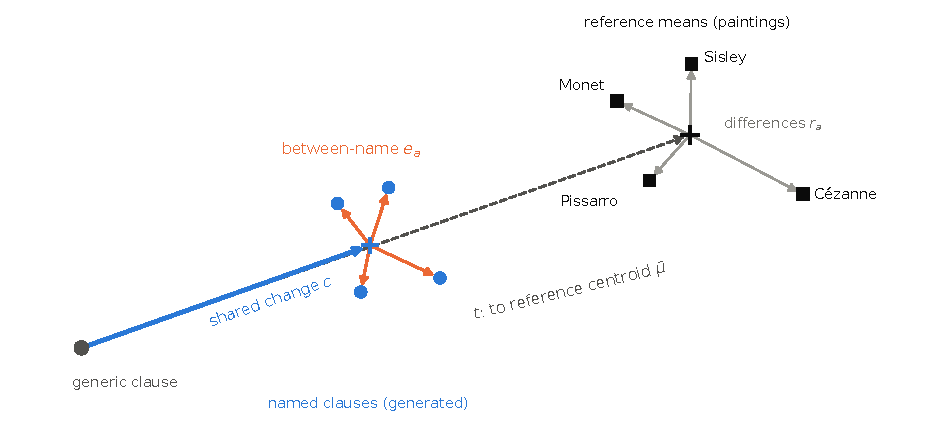
\includegraphics[width=0.92\linewidth]{fig_schematic.pdf}
\caption{The decomposition, drawn schematically (positions are illustrative, not data).
Relative to the generic clause, the four named outputs move by a shared change $c$ and differ
from one another by between-name differences $e_a$. The reference means of the four painters
differ from their centroid $\bar\mu$ by $r_a$. A faithful imitator would move the generic
output all the way along $t$ and reproduce $r_a$; because the painters are close to each other
relative to $\|t\|$, most of that movement would also be shared.}
\label{fig:schematic}
\end{figure}

\section{Related work}\label{sec:related}

\paragraph{Artist style similarity and recognition.}
\citet{somepalli2024style} train contrastive style descriptors (CSD) and score generated images
against averaged artist prototypes. \citet{verma2025imitation} use such style similarity to
estimate how many training images a model needs before it imitates an artist.
\citet{casper2023measuring} classify Stable Diffusion imitations of 70 artists with CLIP and find
them recognizable on average. \citet{su2025prompted} benchmark identifying the prompted artist
across 110 artists, with content-controlled name substitutions and comparisons with the image
generated from the same seed without the artist's name. \citet{moayeri2025rethinking} consider an
artist's style at risk when the artist's own works are recognizable and the style is also
recognized in generated images, which applies to about a fifth of 372 artists.
\citet{frochte2026csd} shows that raw CSD cosine fails to separate same-artist from
different-artist pairs for part of a 91-artist corpus and also evaluates recognition of prompted
generations. \citet{xing2026beyond} observe that artist-grounded generation often falls back on
canonical shortcuts such as generic palettes and recurring motifs. Artist-free comparisons and
closed-set recognition, which uses between-name information, are thus established readouts. We add
a generic-style control, split what the names add into shared and between-name parts, and
benchmark both against the painters' reference collections.

\paragraph{Style mimicry, protection and removal.}
Glaze \citep{shan2023glaze} perturbs artworks to disrupt fine-tuned mimicry, and
\citet{honig2025adversarial} show with a user study that such protections can be bypassed.
Concept erasure \citep{gandikota2023erasing} and concept ablation \citep{kumari2023ablating},
which maps an artist's style onto an anchor concept such as a generic painting, remove styles
from diffusion models, and UnlearnCanvas \citep{zhang2024unlearncanvas} benchmarks such removal.
The generic-painting anchor of concept ablation is close to our generic control.

\paragraph{Change-based readouts and quantitative studies of art.}
Directional CLIP similarity scores the direction of an image change against a text direction
\citep{gal2022stylegannada,brooks2023instructpix2pix}; applied to artist names, it would include
the shared component unless that component is removed. \citet{deliege2025} assess stylistic
imitation with expert raters, AI-Pastiche \citep{asperti2025pastiche} studies authenticity and
prompt adherence of generated paintings, and \citet{fu2025aiwikiart} test vision-language models
on artist attribution and detection of generated paintings. Quantitative art research describes
paintings by color, composition and image statistics \citep{kim2014,sigaki2018,lee2020} and
traces historical change in learned embeddings \citep{kim2026}; our features follow this
tradition. Our estimator is the cross-validated distance of representational similarity analysis
\citep{diedrichsen2017representational}, and conditional evaluation metrics similarly separate
variation within conditions from relations among their means \citep{benny2021conditional}.

\section{Design and measurements}\label{sec:design}

\paragraph{Painters and reference collections.}
The reference collection contains 649 digital reproductions: 297 by Monet, 106 by Sisley, 141 by
Pissarro and 105 by C\'ezanne; four further eligible reproductions could not be measured (one with
a transparent layer, three in unprofiled non-RGB color spaces). Works were eligible if Wikidata records them as paintings by that
painter alone, a fixed lexicon classifies their titles and metadata as outdoor places, and
Wikimedia Commons holds a reproduction at least 1,024 pixels on the short side
\citep{wikimediacommons,vrandecic2014wikidata}. A separate 221-work development panel of the same
painters sets the feature scaling; works were assigned to the two panels by a fixed hash rule
before this experiment. The primary comparisons use only the reference collection; the
development panel appears as an alternative target in sensitivity checks. Three of the painters
are Impressionists who often painted similar motifs, and C\'ezanne's work departs more clearly
from theirs. The collections differ in subject mix (by title, 191 of 297 Monet works are water
scenes, against 31 of 105 for C\'ezanne; a visual audit by AI assistants, not checked by a human,
disagreed with the title-derived class for 230 of 870 works), which we address with
content-matched targets. Painter means receive equal weight throughout.

\paragraph{Prompts.}
Fourteen fixed outdoor scene descriptions cover water, built, land and mixed compositions
(Appendix Table~\ref{tab:scenes}). Each is crossed with six clauses: none; ``Render as an oil
painting.''; and ``Render as an oil painting in the style of Claude Monet.'' (or Alfred Sisley,
Camille Pissarro, Paul Cezanne; the prompts spell C\'ezanne without the accent). The clause
precedes the scene description, and every prompt ends with ``No text or frame.''

\paragraph{Generators.}
All requests went through the OpenRouter image API with one fixed provider per configuration and
fallbacks disabled: \texttt{openai/\allowbreak gpt-\allowbreak image-1} and
\texttt{gpt-\allowbreak image-2} (GPT Image 1 and 2), \texttt{gpt-\allowbreak image-\allowbreak
2.5-\allowbreak flare} and \texttt{gpt-\allowbreak image-\allowbreak 2.5-\allowbreak sunburst}
(Flare and Sunburst), all at medium quality; Nano Banana 2 (\texttt{google/\allowbreak
gemini-\allowbreak 3.1-\allowbreak flash-\allowbreak image}) at 1K resolution; and FLUX.2 Max
(\texttt{black-\allowbreak forest-\allowbreak labs/\allowbreak flux.2-\allowbreak max}). The
gateway's catalogue listed Flare and Sunburst as GPT Image 2.5 variants from the OpenAI provider at
the time of collection; we have no further documentation of how they differ and cannot guarantee
that they remain available. All configurations return $1024\times1024$ images. Each
configuration--scene--clause cell received two separate requests, 1,008 images in total, collected
on 10 September 2026 (UTC) in a randomized order fixed before collection. Responses do not echo
model identifiers, and the explicit routes were not tested with an invalid identifier, so the
labels denote the requested configurations. The images of any two configurations, Flare and
Sunburst included, lie farther apart than each configuration's own repeats in at least 91.7\% of
scene--clause cells in every representation (Appendix~\ref{app:provenance}).
Figure~\ref{fig:examples} shows one scene under all six clauses.

\begin{figure}[t]
\centering
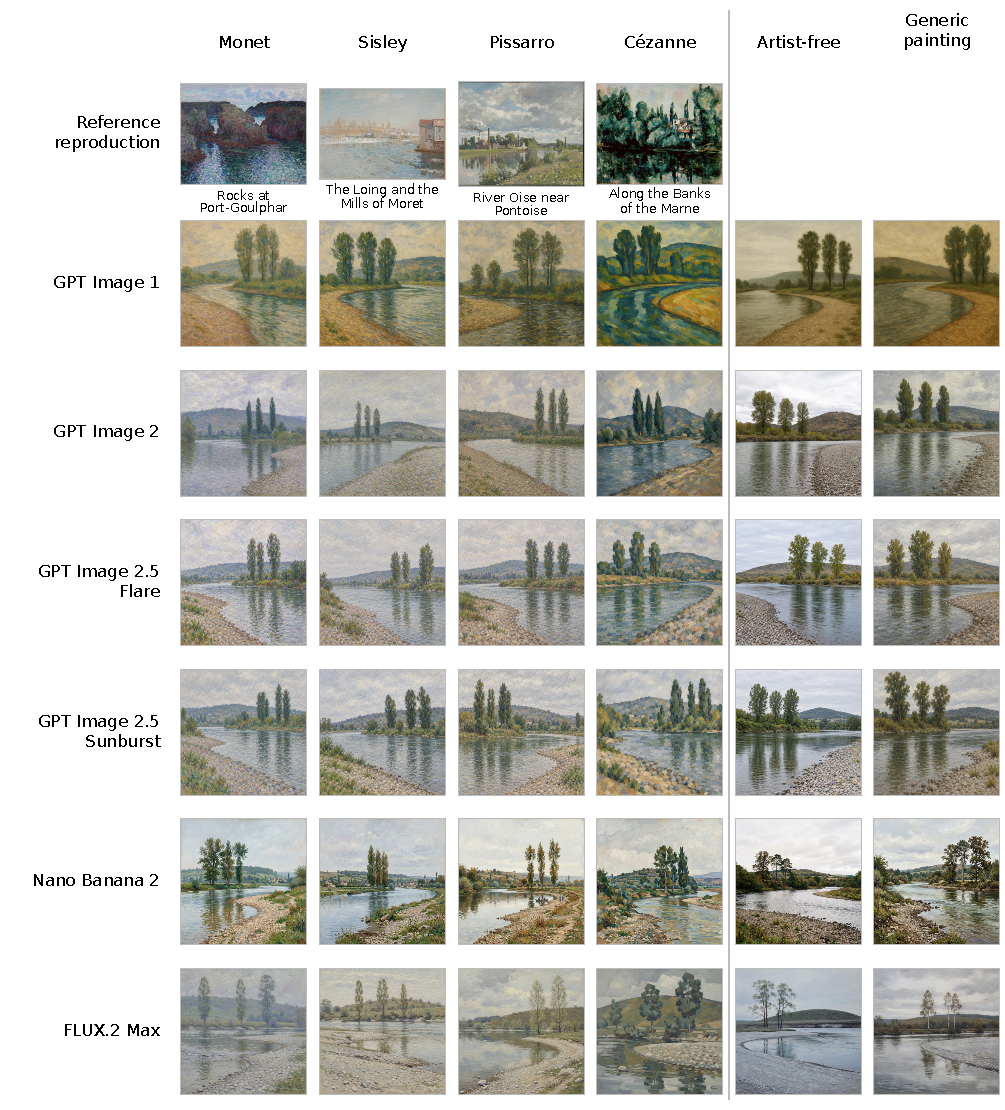
\includegraphics[width=\linewidth]{specificity_original_generated.pdf}
\caption{One scene description (a river bending past a gravel bank, three trees on the far bank
and a low hill under an overcast sky) under all six clauses in each configuration (first repeat,
selected by a fixed rule before inspection); GPT Image 2.5 Flare and Sunburst are abbreviated
Flare and Sunburst elsewhere. The top row shows one public-domain reference reproduction per
painter for orientation (Wikimedia Commons; titles in the panel); references are not matched to
the scene.}
\label{fig:examples}
\end{figure}

\paragraph{Measurements.}
The primary representation has 31 interpretable coordinates in three families: 11 color features
(lightness, chroma, hue concentration and entropy, and color differences at three spatial
scales), 8 spatial features (spectral slope and anisotropy, gradient statistics, orientation
entropy and balance, and quadrant variation) and 12 texture features (wavelet energies,
local-binary-pattern entropies and local contrast); Appendix~\ref{app:features} defines them.
Images are converted to sRGB and resized to a 512-pixel short side. Each coordinate is centered
and scaled by the development panel's painter-weighted median and interquartile range. We also
embed every image with CLIP ViT-L/14 \citep{radford2021} and the released CSD ViT-L checkpoint
\citep{somepalli2024style}, using each encoder's native $224\times224$ center crop and
unit-normalized 768-dimensional outputs (Appendix~\ref{app:learned}). The representations differ
in how well they separate the painters' genuine works: assigning each development work to the
nearest reference mean gives 49.8\% macro accuracy in the 31 features, with only 39.6\% of Monet
and 30.6\% of Sisley works correct, against 79.8\% in CLIP and 79.6\% in CSD. The 31 features
were prespecified for their interpretability, and the embeddings were added afterwards. Embedding
metrics can respond to image content \citep{kynkaanniemi2023role}. CSD was trained with these
painters among its style tags.

\section{Separating shared and between-name change}\label{sec:method}

Three questions organize the quantities below. The shared fraction and its two benchmarks
(Sections~\ref{sec:split}--\ref{sec:benchmarks}) say how much of what the names add is common to
all names. The aligned amplitude $\beta$, the relative size $Q$, the alignment ratio
$\beta/\sqrt{Q}$ and the error $D$, for which 1 means making no painter distinctions
(Section~\ref{sec:agreement-method}), say whether the between-name differences match the painters'
differences in direction and in size. The shared term of an exact identity for proximity
(Section~\ref{sec:proximity}) says how much of the proximity gain is common to all names. Appendix
Table~\ref{tab:estimands} lists the main symbols.

\subsection{The split}\label{sec:split}

Let $z_{sak}$ be one configuration's feature vector for scene $s=1,\dots,S$ ($S=14$), clause $a$
and repeat $k\in\{1,2\}$, where $a$ is f (artist-free), g (generic) or one of the painters
$1,\dots,4$. Averaging over scenes within each repeat gives $\bar z_{ak}$. Relative to the
generic clause, the four named means split into a shared change and between-name differences,
\begin{equation}
\bar z_{ak}-\bar z_{\mathrm{g}k}=c_k+e_{ak},\qquad
c_k=\tfrac14\sum_{a=1}^4\bar z_{ak}-\bar z_{\mathrm{g}k},\qquad
e_{ak}=\bar z_{ak}-\tfrac14\sum_{a'=1}^4\bar z_{a'k},
\label{eq:split}
\end{equation}
with squared sizes
\begin{equation}
N=4\ip{c_1}{c_2},\qquad B=\sum_{a=1}^4\ip{e_{a1}}{e_{a2}}.
\label{eq:components}
\end{equation}
If each repeat equals a fixed mean plus noise with mean zero that is independent between
repeats, these cross-repeat products have the squared means as their expectations, whereas
squaring one repeat would add the noise variance. Estimates can be negative; we keep them. The
\emph{shared fraction} is $N/(N+B)$. The between-name differences do not depend on the baseline;
Appendix~\ref{app:estimators} gives the split against the artist-free baseline.

\subsection{Benchmarks}\label{sec:benchmarks}

Let $\mu_a$ be painter $a$'s mean reference vector, $\bar\mu$ their centroid, $r_a=\mu_a-\bar\mu$,
and $H=\sum_a\|r_a\|^2$ the \emph{reference painter spread}; $B/H$ compares the generated
between-name differences with the reference differences in size. Two benchmarks keep the observed
generic outputs and change what the names do:
\begin{itemize}
\item \textbf{Faithful imitator.} Each named mean equals the painter's reference mean, so the
shared change becomes $t=\bar\mu-\bar z_{\mathrm{g}}$ and the between-name differences $r_a$, with
shared fraction $N^*/(N^*+H)$ and $N^*=4\ip{t_1}{t_2}$. It includes the distance between generated
images and photographed paintings, so it is a reference point rather than a target or a bound;
configurations with small between-name differences can exceed it.
\item \textbf{Exact differences.} The observed shared change is kept and the between-name
differences equal $r_a$, giving $N/(N+H)$. This removes the dependence on how far the generic
outputs are from the paintings; the observed fraction differs from it only through $B/H$
versus 1.
\end{itemize}
The observed fraction differs from the faithful one through two separate quantities: how much of
$t$ the shared change covers, and how large the between-name differences are relative to $H$.
We report the cosine between $c$ and $t$, corrected by cross-repeat products, and the fraction
$\lambda=\ip{c}{t}/\|t\|^2$ of the distance covered along $t$.

\subsection{Agreement with the reference differences}\label{sec:agreement-method}

To test whether the between-name differences match the reference differences, center each scene
separately, $d_{sak}=z_{sak}-\frac14\sum_{a'}z_{sa'k}$, and define
\begin{equation}
\widehat\beta=\frac1S\sum_s\frac{1}{2}\sum_{k=1}^2\frac{\sum_a\ip{d_{sak}}{r_a}}{H},\qquad
\widehat D=\frac1S\sum_s\frac1H\sum_a\ip{d_{sa1}-r_a}{d_{sa2}-r_a};
\label{eq:beta-d}
\end{equation}
we drop the hats below. The aligned amplitude $\beta$ projects the generated differences onto the
reference pattern: $\beta=1$ matches its size along that pattern, and $\beta>0$ indicates a
response in the right direction in aggregate. The error $D$ also counts differences in other
directions: its expectation is 0 for exact agreement, 1 when the names produce no differences, and
$(\kappa-1)^2$ when the reference pattern is reproduced at $\kappa$ times its size. With
$Q=(SH)^{-1}\sum_{s,a}\ip{d_{sa1}}{d_{sa2}}$, the squared size of the generated differences
relative to the reference, $D=1-2\beta+Q$. The prespecified split writes $D$ exactly as the error of
the amplitude along the reference pattern plus an off-pattern part, the size of the differences
orthogonal to it (Appendix~\ref{app:estimators}). The alignment ratio $\beta/\sqrt{Q}$ is the
alignment of the scene-wise differences with the pooled reference pattern: it is unaffected by
rescaling the differences but lowered by off-pattern differences and by their variation across
scenes. Rescaling the differences optimally would leave $D=1-\beta^2/Q$; $D_{\mathrm{held}}$
applies such a rescaling fitted on the other scenes and therefore closely follows the alignment
ratio. Every scene is compared with
the same pooled target, so $D$ also penalizes differences that vary across scenes:
$D=D_{\mathrm{agg}}+V_{\mathrm{scene}}$, where $D_{\mathrm{agg}}$ scores the scene-averaged
differences and $Q=B/H+V_{\mathrm{scene}}$; the scene-averaged alignment is $\beta/\sqrt{B/H}$. Genuine paintings do not reach $D=0$ either when two
works per painter stand in for the two repeats of a scene, so we also report that error for held-out
reference paintings. Specificity here means agreement with the differences between the painters'
reference means in a given representation; no perceptual judgment enters it.

\subsection{Proximity and recognition in embeddings}\label{sec:proximity}

In an embedding, let $g_a$ and $g_{\mathrm{g}}$ be the mean unit embeddings for painter $a$ and the
generic clause and $\mu_a$ the mean of the painter's unit reference embeddings, so that
$g_a^\top\mu_a$ is the mean cosine similarity between named images and the painter's reference
works. The named-minus-generic gain in this similarity decomposes exactly as
\begin{equation}
\underbrace{\frac14\sum_a g_a^\top\mu_a-g_{\mathrm{g}}^\top\bar\mu}_{\text{proximity gain}}
=\underbrace{(\bar g-g_{\mathrm{g}})^\top\bar\mu}_{\text{shared}}
+\underbrace{\frac{H\beta}{4}}_{\text{painter-specific}},
\label{eq:prototype-gain}
\end{equation}
with $H$ and $\beta$ computed in the embedding (Appendix~\ref{app:learned}); with $K$ painters the
painter-specific term is $H\beta/K$. The shared term does
not depend on which name produced which image. The identity holds for any score that is linear in
the image embedding, including cosine similarity to a prototype normalized to unit length; with
normalized prototypes the shares below change by at most 0.5 points
(Appendix Table~\ref{tab:learned-settings}). Readouts based on ranks, maxima or thresholds, such as
retrieval, top-$k$ similarity or imitation decisions, are outside its scope. Raw proximity without a baseline adds
$g_{\mathrm{g}}^\top\bar\mu$, which does not depend on the name either. The faithful benchmark sets
$g_a=\mu_a$; the exact-differences benchmark keeps the shared term and sets the painter-specific
term to $H/4$. The shared term is therefore a majority of the gain of an exact-differences
generator whenever it exceeds $H/4$, that is, whenever the shared movement toward the painters'
common prototype is larger than a quarter of their spread. Recognition is a separate readout: each
named image is assigned to the reference prototype, normalized to unit length, with the largest
cosine similarity, and we report macro accuracy over the four painters.

\subsection{Inference and status of the analyses}\label{sec:inference}

Before collection, the protocol fixed an inferential family of 21 comparisons in the 31 features,
the six aligned amplitudes and the 15 pairwise differences in $D$, with paired-scene Student
intervals and a Bonferroni adjustment across all 21. It also prescribed unadjusted intervals and a
paired-scene bootstrap for the pairwise differences (Appendix Table~\ref{tab:pairs}), resampling of
the reference works within painter, the artist-free shared/between-name split, the split of $D$
along and off the reference pattern, and distribution diagnostics (Appendix
Table~\ref{tab:diversity}); its scene fixed-effects regression reproduces the pairwise differences,
and a projection of the means (Appendix Figure~\ref{fig:projection}) replaces its reference PCA
display of full distributions. All other intervals are unadjusted: paired-scene Student intervals
for per-scene statistics and percentile intervals for resampled ones. We call a difference
\emph{resolved} when its interval excludes the comparison value; only the 21 prespecified
comparisons use adjusted intervals, and comparisons of $D$ with 1 lie outside that family. The
protocol ranked configurations only on $D$; the alignment ratio, $D_{\mathrm{held}}$ and their
resampling were defined after collection, when the $D$ rankings were known to depend on the
representation. The
intervals describe the 14 authored scenes and the finite reference panels, not new scenes or
painters. A first collection attempt was stopped before any image was measured, when a gateway
route accepted an invalid model identifier, and the scene panel was then reduced from 16 to 14
descriptions to fit the budget (Appendix~\ref{app:provenance}). Everything else, including the
generic-baseline split, the benchmarks, the embedding analyses, recognition, the genuine-painting
controls and the resampling of these quantities, was added afterwards under written plans on images
whose other results were known; the plans, included in the supplementary material, record which
values were already known when each was written. These analyses are descriptive.

\section{Results}\label{sec:results}

All 1,008 images yielded valid measurements. Ranges, differences and shares are computed from
unrounded values.

\subsection{Most of what the names add is shared, and faithful imitation would share even more}\label{sec:shared}

% Generated by paper/tmlr/build_assets.py; do not edit by hand.
% input reports/painter_tmlr_diagnostics_v1/analysis.json sha256 76792fa35f90e3d8fec1a75b0eec27d69cac14ed875fce8b64096b8e2525a4d4
% input reports/painter_tmlr_diagnostics_v2/analysis.json sha256 bed891f767a98f4b281b6783b1021956f4d2c3ff80becbf6b2693ee45987ef1a
\begin{table}[t]
\caption{Shared fraction $N/(N+B)$ of what the four names add beyond the generic clause (31 features), with a 95\% interval from 5,000 scene resamples, and the squared sizes of the shared change ($N$) and of the between-name differences ($B$) relative to the reference painter spread $H$. Faithful: the fraction if each named mean equalled the painter's reference mean, from the same generic outputs. Exact differences: the fraction if the observed shared change were kept and $B/H$ were 1, $N/(N+H)$. Obs.$<$faithful: share of scene resamples in which the observed fraction is below the faithful one. Appendix Table~\ref{tab:direction} gives the direction of the shared change.}
\label{tab:shared}
\vspace{2pt}
\centering\small\setlength{\tabcolsep}{4pt}
\begin{tabular}{@{}lrcrrrrr@{}}
\toprule
 & \multicolumn{4}{c}{Observed} & \multicolumn{3}{c}{Benchmarks}\\
\cmidrule(lr){2-5}\cmidrule(l){6-8}
Configuration & fraction (\%) & scene 95\% & $N/H$ & $B/H$ & faithful (\%) & exact diff.\ (\%) & obs.$<$faithful (\%)\\
\midrule
GPT Image 1 & 71.3 & [67.6, 74.9] & 5.26 & 2.12 & 95.2 & 84.0 & 100.0\\
GPT Image 2 & 70.9 & [66.5, 75.6] & 4.98 & 2.04 & 89.3 & 83.3 & 100.0\\
Flare & 71.1 & [66.7, 76.7] & 4.99 & 2.03 & 84.8 & 83.3 & 100.0\\
Sunburst & 66.7 & [63.3, 71.1] & 3.97 & 1.98 & 86.9 & 79.9 & 100.0\\
Nano Banana 2 & 69.1 & [52.0, 75.8] & 1.36 & 0.61 & 92.5 & 57.6 & 100.0\\
FLUX.2 Max & 88.4 & [76.8, 94.2] & 5.34 & 0.70 & 90.4 & 84.2 & 84.1\\
\bottomrule
\end{tabular}
\end{table}


Beyond the generic clause, 66.7--88.4\% of the squared change that the names add is shared by all
four names (Table~\ref{tab:shared}). A faithful imitator starting from the same generic outputs
would show 84.8--95.2\% (Figure~\ref{fig:benchmark}): the generic outputs are much farther from the
paintings than the four painters are from each other, so most of any faithful movement toward them
is shared. The observed fraction is below the faithful one in every scene resample for five
configurations; for FLUX.2 Max it is below in 84.1\% of resamples, and its interval [76.8, 94.2]
includes the faithful value.

The exact-differences benchmark removes the distance to the paintings from the comparison. A
generator that kept each configuration's shared change but reproduced the painter differences
exactly would show 57.6--84.2\%, so even perfect between-name differences would leave most of the
change shared in every configuration. The observed fraction differs from this benchmark only
through the size of the between-name differences: $B/H$ is 1.98--2.12 for the four GPT
configurations, whose fractions are therefore below the benchmark, and 0.61--0.70 for Nano Banana 2
and FLUX.2 Max, whose fractions are above it. Being below the faithful value therefore does not
mean being more specific. Nano Banana 2, for example, is far below its faithful value because its
shared change covers only 24.8\% of the distance to the reference centroid; with exact painter
differences its fraction would fall to 57.6\%.

The shared change points toward the reference centroid, with corrected cosine 0.57--0.86 (Appendix
Table~\ref{tab:direction}). For Nano Banana 2 and FLUX.2 Max, 55.5\% and 52.8\% of its squared size
also lies along the artist-free-to-generic shift, against 0.1--22.0\% for the four GPT
configurations, so in those two configurations part of what a name adds continues the generic
painting instruction. Computed within scenes, the shared fraction is 52.8--93.6\%, and against the
artist-free baseline, which includes the painting instruction, 82.5--95.7\% (Appendix~\ref{app:hand}).

\begin{figure}[t]
\centering
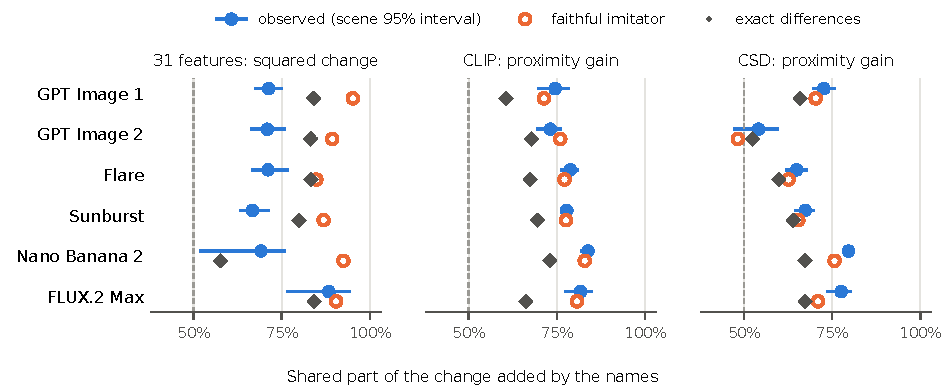
\includegraphics[width=\linewidth]{fig_benchmark.pdf}
\caption{Shared part of what the four names add beyond the generic clause (filled, with 95\%
intervals from scene resampling), with the values a faithful imitator (open) and an
exact-differences generator (diamond) would show. Left: squared change in the 31 features. Middle
and right: share of the proximity gain in the embeddings (Equation~\ref{eq:prototype-gain}). The
squared change counts all between-name differences, including those off the reference pattern,
whereas the proximity gain counts only their aligned part, $H\beta/4$; this is why the observed
values lie below the faithful ones on the left but mostly at or above them in the embeddings (Appendix
Table~\ref{tab:learned-squared} gives the squared-change shares in the embeddings). In the embeddings
the faithful benchmark also inherits the variety of the reference works, whose mean embeddings are
shorter than those of the generated images, markedly so in CSD. The dotted line marks 50\%.}
\label{fig:benchmark}
\end{figure}

\subsection{Proximity gain mostly measures the shared change}\label{sec:learned}

% Generated by paper/tmlr/build_assets.py; do not edit by hand.
% input reports/painter_tmlr_diagnostics_v2/analysis.json sha256 bed891f767a98f4b281b6783b1021956f4d2c3ff80becbf6b2693ee45987ef1a
\begin{table}[t]
\caption{Shared part (\%) of the named-minus-generic proximity gain in CLIP and CSD (Equation~\ref{eq:prototype-gain}), with a 95\% interval from 5,000 scene resamples. Faithful: the same share if every named mean embedding equalled the painter's mean reference embedding. Exact differences: the share if the observed shared term were kept and the painter-specific term had its reference value $H/4$.}
\label{tab:learned}
\vspace{2pt}
\centering\small\setlength{\tabcolsep}{3.5pt}
\begin{tabular}{@{}lrcrrrcrr@{}}
\toprule
 & \multicolumn{4}{c}{CLIP} & \multicolumn{4}{c}{CSD}\\
\cmidrule(lr){2-5}\cmidrule(l){6-9}
Configuration & obs. & scene 95\% & faithful & exact diff. & obs. & scene 95\% & faithful & exact diff.\\
\midrule
GPT Image 1 & 74.5 & [69.9, 78.2] & 71.3 & 60.6 & 72.7 & [69.7, 75.6] & 70.4 & 66.0\\
GPT Image 2 & 73.2 & [69.7, 75.9] & 76.0 & 67.7 & 54.2 & [47.4, 59.3] & 48.3 & 52.5\\
Flare & 78.8 & [76.4, 80.7] & 77.1 & 67.5 & 65.0 & [62.1, 67.6] & 62.7 & 59.9\\
Sunburst & 77.7 & [76.3, 79.2] & 77.6 & 69.4 & 67.4 & [64.6, 69.6] & 65.4 & 64.0\\
Nano Banana 2 & 83.8 & [82.0, 85.3] & 82.9 & 73.0 & 79.7 & [78.5, 80.8] & 75.7 & 67.3\\
FLUX.2 Max & 81.7 & [77.4, 84.9] & 80.7 & 66.2 & 77.6 & [73.7, 80.3] & 71.0 & 67.4\\
\bottomrule
\end{tabular}
\end{table}

% Generated by paper/tmlr/build_assets.py; do not edit by hand.
% input reports/painter_learned_audit_v1/analysis.json sha256 06c77de4be133afc203dda122b2816d4f866e1389999f18bc94b3d9c668f28f7
% input reports/painter_tmlr_diagnostics_v5/analysis.json sha256 5747902e4fae5ff111a52b5f2b8da112bc26c611555e82314b278de953981f6b
\begin{table}[t]
\caption{Readouts of the same images in each embedding. Proximity: named-minus-generic gain in mean cosine similarity to the prompted painter's reference works, split by Equation~\ref{eq:prototype-gain} into the shared term and the painter-specific term $H\beta/4$. Recognition: macro accuracy of assigning each of the 112 named images to its prompted painter by the nearest reference prototype (chance 25\%). Agreement: alignment ratio (higher is better) and error $D$ (lower is better); Table~\ref{tab:agreement} gives the 31-feature values. Bold marks the largest value in each column and embedding (the lowest for $D$); Appendix Table~\ref{tab:stability} shows how often each configuration is best under scene resampling.}
\label{tab:readouts}
\vspace{2pt}
\centering\small
\begin{tabular}{@{}lrrrrrr@{}}
\toprule
 & \multicolumn{3}{c}{Proximity gain} & Recognition & \multicolumn{2}{c}{Agreement}\\
\cmidrule(lr){2-4}\cmidrule(l){6-7}
Configuration & total & shared & painter-specific & (\%) & $\beta/\sqrt{Q}$ & $D$\\
\midrule
\multicolumn{7}{@{}l}{\textit{CLIP}}\\
GPT Image 1 & 0.072 & 0.053 & 0.018 & 60.7 & 0.555 & \textbf{0.847}\\
GPT Image 2 & 0.100 & 0.073 & \textbf{0.027} & \textbf{68.8} & \textbf{0.609} & 1.061\\
Flare & 0.091 & 0.072 & 0.019 & 59.8 & 0.515 & 1.057\\
Sunburst & 0.101 & 0.079 & 0.023 & 58.9 & 0.543 & 1.136\\
Nano Banana 2 & \textbf{0.112} & 0.094 & 0.018 & 51.8 & 0.493 & 1.078\\
FLUX.2 Max & 0.083 & 0.068 & 0.015 & 41.1 & 0.453 & 1.058\\
\midrule
\multicolumn{7}{@{}l}{\textit{CSD}}\\
GPT Image 1 & \textbf{0.217} & 0.158 & 0.059 & 72.3 & 0.667 & 0.735\\
GPT Image 2 & 0.166 & 0.090 & \textbf{0.076} & \textbf{75.9} & \textbf{0.737} & 0.741\\
Flare & 0.187 & 0.121 & 0.065 & 62.5 & 0.673 & 0.819\\
Sunburst & 0.214 & 0.144 & 0.070 & 61.6 & 0.666 & 0.944\\
Nano Banana 2 & 0.210 & 0.167 & 0.043 & 50.9 & 0.513 & 0.999\\
FLUX.2 Max & \textbf{0.217} & 0.168 & 0.049 & 39.3 & 0.627 & \textbf{0.714}\\
\bottomrule
\end{tabular}
\end{table}


In CLIP and CSD, the shared term of Equation~\ref{eq:prototype-gain} supplies 73.2--83.8\% and
54.2--79.7\% of the named-minus-generic proximity gain (Table~\ref{tab:learned}). A faithful
imitator would obtain 71.3--82.9\% and 48.3--75.7\% of its gain from the same term; the observed
shares differ from these by $-$2.8 to +6.5 percentage points and are above them for all six
configurations in CSD. With exact painter differences instead, the shared term would still supply
60.6--73.0\% (CLIP) and 52.5--67.4\% (CSD) of the gain, because the shared movement toward the four
painters' common prototype exceeds a quarter of their spread in every case. The shared term is a
majority of the gain, with a scene interval above 50\%, in 11 of the 12 configuration--encoder pairs.
The exception is GPT Image 2 in CSD, at 54.2\% [47.4, 59.3], where a faithful imitator would obtain
48.3\%. For individual painters, C\'ezanne's gain is the least shared in 11 of the 12 pairs, as low
as 34.6\% (Appendix Table~\ref{tab:per-painter}). Using the audited source regions or the
development panel as the reference target changes the observed shares by at most 1.6 points
(Appendix Table~\ref{tab:learned-settings}).

The shared term also drives the differences in gain between configurations, which is how proximity
is used to compare models (Table~\ref{tab:readouts}). Across the six configurations, the gain
correlates with its shared term at 0.96 [0.91, 0.98] in CLIP and 0.95 [0.79, 0.99] in CSD (95\%
intervals from scene resampling), and the shared term varies more across configurations than the
painter-specific term, by a factor of 11 [4.6, 29.3] in CLIP and 5.8 [2.5, 13.8] in CSD (in
variance). With six configurations and the gain being the sum of the two terms, these are
descriptive. In CLIP the gain ranks the configurations exactly as its shared term does; in CSD it
correlates $-$0.65 with the painter-specific term. Nano Banana 2 has the largest CLIP gain but the
fifth-largest painter-specific term, and GPT Image 2 has the smallest CSD gain but the largest
painter-specific term.

\subsection{Between-name differences point the right way; their size varies}\label{sec:agreement}

% Generated by paper/tmlr/build_assets.py; do not edit by hand.
% input reports/painter_specificity_v2/psv2-20260911/models.csv sha256 eed121f77626d8a37235b5bb19e370e3fbd7b6bae44b559d1b866e27e9cac41c
% input reports/painter_specificity_review_v1/analysis.json sha256 2fabb78e15dfcc7b027a73170f6ad0c87af0196c754b4e6f45275269c2c961e2
% input data/manifests/painter_specificity_v2/psv2-20260911/analysis.json sha256 c1d21b16f840a10fd253c1d558743a09671acf3d4e48601ddcc96625a5a90be0
% input reports/painter_tmlr_diagnostics_v2/analysis.json sha256 bed891f767a98f4b281b6783b1021956f4d2c3ff80becbf6b2693ee45987ef1a
\begin{table}[t]
\caption{Agreement of the between-name differences with the reference painter differences (31 features). $\beta=1$ matches the reference pattern's size along its direction; $Q$ is the squared size of the generated differences relative to the reference, and $\beta/\sqrt{Q}$ their alignment with the reference pattern, unaffected by rescaling the differences (1 for a scaled copy of the reference pattern); $D=1-2\beta+Q$ is 0 for exact agreement and 1 when names produce no differences. Scenes: for $\beta$, prespecified 95\% simultaneous Student intervals over 21 endpoints; for $D$, unadjusted 95\% Student intervals. References: prespecified 95\% percentile intervals from resampling reference works within painter; resampling adds a second finite-sample bias to $H$, so these intervals for $\beta$ lie slightly low. $D<1$: share of 2,000 joint resamples of scenes and reference works with $D$ below 1.}
\label{tab:agreement}
\vspace{2pt}
\centering\small\setlength{\tabcolsep}{3pt}
\begin{tabular}{@{}lrccrrrccr@{}}
\toprule
 & \multicolumn{3}{c}{Aligned amplitude $\beta$} & & & \multicolumn{4}{c}{Error $D$}\\
\cmidrule(lr){2-4}\cmidrule(l){7-10}
Configuration & est. & scenes & references & $Q$ & $\beta/\sqrt{Q}$ & est. & scenes & references & $D<1$ (\%)\\
\midrule
GPT Image 1 & 0.938 & [0.709, 1.168] & [0.767, 0.989] & 2.449 & 0.600 & 1.572 & [1.129, 2.016] & [1.260, 1.892] & 0.7\\
GPT Image 2 & 0.999 & [0.893, 1.104] & [0.804, 1.067] & 2.223 & 0.670 & 1.226 & [0.957, 1.495] & [0.976, 1.507] & 9.9\\
Flare & 0.772 & [0.680, 0.864] & [0.568, 0.878] & 2.281 & 0.511 & 1.738 & [1.477, 1.999] & [1.407, 2.032] & 0.0\\
Sunburst & 0.824 & [0.680, 0.968] & [0.620, 0.929] & 2.289 & 0.545 & 1.641 & [1.312, 1.971] & [1.318, 1.925] & 0.1\\
Nano Banana 2 & 0.442 & [0.256, 0.629] & [0.342, 0.499] & 0.994 & 0.444 & 1.109 & [0.582, 1.636] & [0.961, 1.266] & 33.4\\
FLUX.2 Max & 0.470 & [0.239, 0.701] & [0.369, 0.509] & 0.741 & 0.546 & 0.801 & [0.586, 1.016] & [0.693, 0.945] & 94.2\\
\bottomrule
\end{tabular}
\end{table}


\paragraph{Direction.} Every configuration responds in the reference direction
(Table~\ref{tab:agreement}). In the 31 features all six aligned amplitudes are 0.442--0.999, with
prespecified scene intervals above zero and reference-resampling lower bounds of at least 0.342; in
the embeddings they are 0.438--0.936, all with scene intervals above zero (Appendix
Table~\ref{tab:embedding-calibration}). By the alignment ratio, GPT Image 2 is best in all
three representations: its alignment ratios are 0.670, 0.609, 0.737 (31 features, CLIP, CSD), the
highest in 98.0\%, 99.7\% and 100.0\% of scene resamples. It also has the lowest error after a
held-out rescaling in each (Tables~\ref{tab:calibration} and~\ref{tab:embedding-agreement}), which
largely restates the alignment ratio, and the highest scene-averaged alignment,
$\beta/\sqrt{B/H}$, at 0.699, 0.711, 0.782. Across the six configurations, the alignment ratio
orders them similarly in the three representations (Spearman 0.60--0.77, against $-$0.14 to 0.66
for $D$). One painter pair points the wrong way: Sunburst's
Monet--Sisley amplitude in the features is $-$0.249 with scene interval [$-$0.369, $-$0.140], although
its reference interval includes zero (Appendix Table~\ref{tab:pair-intervals}).

\paragraph{Size and the error $D$ in the 31 features.} GPT Image 1, Flare and Sunburst have errors
above 1 under both kinds of resampling (lowest interval bounds 1.129 for scenes and 1.260 for
references). Along the reference pattern their amplitude is close to the reference ($\beta=$
0.772--0.938), but 96.9--98.2\% of their error lies off the pattern (Appendix
Table~\ref{tab:calibration}): the names add differences that the painters' reference works do not
show. GPT Image 2's error of 1.226, with intervals that include 1, is likewise almost entirely off
the pattern. FLUX.2 Max and Nano Banana 2 respond less along the pattern and have smaller
off-pattern parts (62.0\% and 71.5\% of their errors). FLUX.2 Max has the lowest error, $D=0.801$,
below 1 in 94.2\% of joint scene and reference resamples (next, Nano Banana 2 at 33.4\%), but its
agreement rests mainly on the C\'ezanne contrast: without C\'ezanne its amplitude is 0.096, its
amplitudes for the three Impressionist pairs are 0.02--0.17, and its Monet--Sisley and
Monet--Pissarro pair errors are 1.16 and 1.51 (Appendix Table~\ref{tab:coverage} and
Figure~\ref{fig:pairs}). Within the prespecified family, two of the 15 pairwise differences are
resolved: Flare and Sunburst have higher error than FLUX.2 Max (unadjusted, 6 of 15 by Student
intervals and 8 by the paired-scene bootstrap; Appendix Table~\ref{tab:pairs}). The comparisons with
1 assume independent repeats: with a Bonferroni adjustment over the six configurations, GPT Image
1's interval for $D$, [0.935, 2.210], includes 1, and its error would fall to 1 if the two repeats
shared a fraction 0.22 of their noise power, against 0.64 for Flare and 0.52 for Sunburst
(Appendix~\ref{app:provenance}).

% Generated by paper/tmlr/build_assets.py; do not edit by hand.
% input reports/painter_tmlr_diagnostics_v3/analysis.json sha256 2aa36a87cd6d23ee909cdf94bd9f512d5743138f1d8a8f7c236d56f33fbceb57
% input reports/painter_tmlr_diagnostics_v4/analysis.json sha256 67431bd384586f294651136b214b9649cfd911059133ec79181eec7527d6b67b
% input reports/painter_tmlr_diagnostics_v5/analysis.json sha256 5747902e4fae5ff111a52b5f2b8da112bc26c611555e82314b278de953981f6b
\begin{table}[t]
\caption{Agreement of the between-name differences with the reference differences in the embeddings. $\beta/\sqrt{Q}$ (alignment ratio) and $D_{\mathrm{held}}$ (error after a held-out rescaling) are unaffected by rescaling the differences; bold marks the best in each embedding. Scenes: unadjusted paired-scene Student 95\% intervals, as for $D$ in Table~\ref{tab:agreement}. $D<1$: share of 2,000 joint scene and reference resamples. 11 scenes: $D$ on the non-mixed scenes against the pooled target and against title-derived content-class targets.}
\label{tab:embedding-agreement}
\vspace{2pt}
\centering\small\setlength{\tabcolsep}{3.5pt}
\begin{tabular}{@{}lrrrrcrrrr@{}}
\toprule
 & & & & \multicolumn{3}{c}{Error $D$} & & \multicolumn{2}{c}{11 scenes}\\
\cmidrule(lr){5-7}\cmidrule(l){9-10}
Configuration & $\beta$ & $Q$ & $\beta/\sqrt{Q}$ & est. & scenes & $D<1$ (\%) & $D_{\mathrm{held}}$ & pooled & class\\
\midrule
\multicolumn{10}{@{}l}{\textit{CLIP}}\\
GPT Image 1 & 0.527 & 0.900 & 0.555 & 0.847 & [0.746, 0.947] & 99.9 & 0.694 & 0.886 & 0.904\\
GPT Image 2 & 0.770 & 1.602 & \textbf{0.609} & 1.061 & [0.905, 1.217] & 21.1 & \textbf{0.631} & 1.067 & 1.091\\
Flare & 0.558 & 1.173 & 0.515 & 1.057 & [0.947, 1.167] & 14.4 & 0.735 & 1.059 & 1.074\\
Sunburst & 0.651 & 1.439 & 0.543 & 1.136 & [1.047, 1.225] & 0.1 & 0.705 & 1.163 & 1.200\\
Nano Banana 2 & 0.523 & 1.124 & 0.493 & 1.078 & [0.918, 1.238] & 15.8 & 0.759 & 1.107 & 1.103\\
FLUX.2 Max & 0.438 & 0.933 & 0.453 & 1.058 & [0.935, 1.182] & 16.4 & 0.796 & 1.019 & 1.023\\
\midrule
\multicolumn{10}{@{}l}{\textit{CSD}}\\
GPT Image 1 & 0.728 & 1.192 & 0.667 & 0.735 & [0.629, 0.842] & 100.0 & 0.557 & 0.778 & 0.767\\
GPT Image 2 & 0.936 & 1.612 & \textbf{0.737} & 0.741 & [0.652, 0.830] & 100.0 & \textbf{0.458} & 0.750 & 0.759\\
Flare & 0.804 & 1.428 & 0.673 & 0.819 & [0.771, 0.867] & 100.0 & 0.547 & 0.819 & 0.804\\
Sunburst & 0.860 & 1.664 & 0.666 & 0.944 & [0.852, 1.037] & 80.8 & 0.556 & 0.933 & 0.930\\
Nano Banana 2 & 0.526 & 1.051 & 0.513 & 0.999 & [0.850, 1.148] & 51.3 & 0.739 & 0.976 & 0.971\\
FLUX.2 Max & 0.598 & 0.910 & 0.627 & 0.714 & [0.609, 0.818] & 100.0 & 0.610 & 0.708 & 0.699\\
\bottomrule
\end{tabular}
\end{table}


\paragraph{The error $D$ in the embeddings.} The embeddings order the configurations differently
(Table~\ref{tab:embedding-agreement}). In CLIP, GPT Image 1 has the lowest error, 0.847 [0.746,
0.947], and only Sunburst's interval, [1.047, 1.225], lies above 1, a verdict that would reverse at
a repeat correlation of 0.14; every CLIP scene-averaged error is below 1 (0.587--0.798), so the CLIP
errors above 1 come from variation across scenes. In CSD the errors are 0.714--0.999; four intervals lie entirely below
1 and none above, and dependence between repeats would only lower them. Content matching on the
reference side does not explain the difference: on the 11 non-mixed scenes, title-derived
content-class targets change the embedding errors by at most 0.037 relative to the pooled target on
the same scenes and keep their order. Because the alignment ratio orders the configurations
similarly across representations, the representations differ mainly in how they weigh the size and
scene variation of the between-name differences; we therefore do not rank the configurations by $D$
across representations.

\paragraph{Genuine paintings.} Held-out reference paintings sampled like the generated images, two
distinct works per painter and pseudo-scene scored against a target from the other half of each
collection, have mean errors of 0.125--0.328 in the 31 features and 0.060--0.216 in the embeddings
(Appendix Table~\ref{tab:genuine}). Their pseudo-scenes have no fixed content, so the pooled
control's expected error is the noise of its half-size target alone (Appendix~\ref{app:hand}),
whereas the generated errors also contain the variation of the differences across scenes. In the
embeddings, where no genuine split exceeds 1, every configuration errs clearly more than genuine
paintings. In the 31 features, genuine splits vary so widely that their central 95\% ranges end at
1.16--1.36 and 5.1--9.1\% of them exceed 1, so the control discriminates weakly there.

\paragraph{Aggregation and scale.} Scoring the scene-averaged differences gives Nano Banana 2 a
lower error than FLUX.2 Max, 0.723 against 0.761, because Nano Banana 2's differences vary more
across scenes. Shrinking each configuration's differences by one scalar fitted on the other 13
scenes removes much of the off-pattern part along with any excess amplitude, brings every error
below 1 and orders the configurations roughly by alignment ratio: GPT Image 2 is lowest at 0.554,
followed by GPT Image 1 (0.645) and Sunburst (0.706), all below FLUX.2 Max's 0.714 (Appendix
Table~\ref{tab:calibration}). Part of the size of the differences may reflect a difference in scale
between clean generated images and photographed paintings, which the alignment ratio ignores.

\subsection{Readouts disagree where they weigh size differently}\label{sec:readouts}

Table~\ref{tab:readouts} places the readouts of the same images side by side, and Appendix
Table~\ref{tab:stability} shows how often each configuration is best when the 14 scenes are
resampled. Within CLIP alone, Nano Banana 2 has the largest proximity gain, 0.112, in 85.8\% of
resamples, yet its prompted names are recognized in 51.8\% of images; GPT Image 2 has the best
recognition, 68.8\%, in 98.7\%; and GPT Image 1 has the lowest error, 0.847, in 99.3\%. Across
representations, FLUX.2 Max has the lowest 31-feature error in 84.7\% of resamples but the least
recognizable names, 41.1\% in CLIP and 39.3\% in CSD, below Nano Banana 2 in 99.9\% of resamples for
both encoders. Other orderings are not stable: in CSD, GPT Image 1 and FLUX.2 Max share the largest
gain (0.217), and no configuration has the largest gain in more than 33.6\% of resamples or the
lowest error in more than 47.2\%.

The disagreements follow from what each readout weighs. Proximity follows the shared change
(Section~\ref{sec:learned}). Across the six configurations, recognition rises with the alignment
ratio (Spearman 0.94 in CLIP and 0.89 in CSD): both reward differences in the right direction,
although recognition also depends on the size of the differences relative to the spread of
individual images and on shared offsets (below). $D$ departs from both because it also penalizes
size, so it favors small differences, as in FLUX.2 Max, over large ones with off-pattern parts.

A shared offset can also change recognition without changing any painter difference. One fixed
translation that aligns the mean of the generated named images with the mean of the reference
prototypes, fitted on the other 13 scenes without painter labels, leaves all centered differences
unchanged but changes recognition by $-$5.4 to +12.5 percentage points in CLIP and +0.9 to +26.8 in
CSD (Appendix~\ref{app:transfer}).

\subsection{Feature families and sensitivity}\label{sec:sensitivity}

\paragraph{Feature families.} Averaged over configurations, the shared fraction is 74.3\% in color,
71.5\% in spatial and 68.2\% in texture features, but the exact-differences benchmark is also lower
for texture (74.7\%, against 77.8\% for color and 79.1\% for spatial), and every family lies 3.6--7.6
points below its benchmark (Appendix Table~\ref{tab:families}). The texture--color difference of
$-$6.1 points [$-$13.5, $-$2.0] is therefore partly expected from the reference differences, and the
texture--spatial ordering is not resolved (texture lower in 65.2\% of paired scene resamples). GPT
Image 1's texture fraction, 48.6\%, the only value below 50\%, comes from oversized texture
differences ($B/H=$ 3.11; exact-differences value 74.6\%). An earlier collection of 2,000 SD-Turbo
images with a different template and seed design shares 64.2\% of the change across all features
and 36.6\% in texture, against faithful and exact-differences values of 92.5\% and 67.4\% overall
(Appendix~\ref{app:sdturbo}); it reuses the references and serves as a retrospective check.

\paragraph{Reference sources.} The shared fraction does not depend on the reference collection; its
benchmarks and the agreement scores do. AI assistants audited all 870 reference and development
reproductions and cropped peripheral artifacts such as frames and calibration strips from 131 of
them; the crops were not verified by a human. With the cropped regions and the original feature
scaling, FLUX.2 Max's error becomes 0.832, all six aligned amplitudes remain above zero, and of the
pairwise differences only Flare--FLUX.2 Max remains resolved. After also refitting the feature
scaling, FLUX.2 Max's error is 0.872, the amplitudes remain above zero, and Flare--FLUX.2 Max and GPT
Image 1--FLUX.2 Max are resolved.

\paragraph{Other checks.} FLUX.2 Max keeps the lowest 31-feature error estimate under every
single-scene deletion, square measurement windows, content-matched reference targets, both
alternative feature weightings and both source corrections (Appendix Table~\ref{tab:sensitivity}),
but in texture features alone Nano Banana 2 is lower, 0.886 against 0.906 (Appendix
Table~\ref{tab:family-agreement}). Correcting the reference spread $H$ for its finite-sample bias
(6.7\%) scales $\beta$, $Q$ and $D-1$ by the same factor: the aligned amplitudes become
0.474--1.071, FLUX.2 Max's error 0.787, no ordering changes, and the exact-differences fractions
rise to 59.3--85.1\% (Appendix Table~\ref{tab:robustness}). The named images of every configuration
are less varied than the painter's reference works (trace ratios 0.25--0.88), and they are closer
to the painter's works than the generic images in 21 of 24 configuration--painter combinations
(Appendix Table~\ref{tab:diversity}).

\section{Discussion}\label{sec:discussion}

\paragraph{What the shared change is.}
The shared change points toward the centroid of these reference reproductions in the 31 features
and increases similarity to their average prototype in both embeddings. Toward that centroid a
faithful imitator would move even further, so a large shared fraction is expected for related
painters and says little about specificity. For Nano Banana 2 and FLUX.2 Max, about half of the
shared change also continues the generic painting instruction. The centroid carries the properties
of old, photographed paintings as well as the painters' common style, and our design cannot tell
movement toward these painters from a generic effect that any artist name would have; a prompt set
with stylistically distant painters, a fictitious name or a clause naming the group
(``Impressionist'') would. The intervention identifies differences between prompt conditions; their
causes inside the generators remain open.

\paragraph{Recommendations for artist-style evaluation.}
First, check that the representation separates the painters' genuine works, and read specificity
from the between-name differences in each representation used. Report direction and size
separately: $\beta$, $Q$, the alignment ratio and $D$ with its split along and off the reference
pattern, with scene and reference intervals, per painter pair as well as in aggregate, and compare
$D$ with genuine paintings sampled the same way, with distinct works. A configuration with $D$ above
1 makes painter differences that are, on balance, farther from the reference than making none; the
split shows whether that comes from the amplitude along the pattern or from differences off it, and
the alignment ratio is unaffected by a difference in scale between generated images and
photographed paintings. Second, when reporting proximity, its gain or a shared fraction, give the
exact-differences and faithful benchmarks, which require only a generic-style control and the
reference means; a shared term larger than a quarter of the painter spread will dominate the
proximity gain whenever $\beta\le1$. Third, match the
reference target to the content of the prompts where possible, and state whether errors are scored
per scene or after averaging, since the aggregation changed the ordering here. Fourth, treat
recognition as its own readout, report how stable rankings are under scene resampling, and note
that recognition responds to shared offsets that leave every painter difference unchanged. None of
these readouts has been validated against perceptual or expert judgments or against a positive
control with known painter differences.

\section{Limitations}\label{sec:limitations}

\paragraph{Scope.} The main experiment uses four related painters, one clause template, 14 authored
scenes and two repeats per cell, and four of the six configurations are OpenAI variants. The
findings describe these painters and configurations. The faithful benchmark mixes painter style with
differences in content and image formation between generated images and photographed paintings; the
exact-differences benchmark avoids this but assumes the observed shared change.

\paragraph{Targets.} Specificity is operationalized as agreement with the differences between
reference means in a chosen representation. Our targets are digital reproductions measured by 31
features and two related encoders, and the errors differ between them. None of these establishes
perceived painter resemblance, and we report no human evaluation. The 31 features separate Monet
and Sisley poorly even for genuine paintings. The reference collections mix the paintings'
properties with subject choices and reproduction processes; the source audit addresses visible
peripheral regions only and was not verified by a human.

\paragraph{Services and inference.} The six configurations are closed services whose checkpoints
we cannot verify, and we cannot tell whether they rewrite prompts. Two repeats cannot establish that
repeated requests are independent. If they shared an error component, the cross-repeat products
would retain it, so $N$, $B$ and $D$ would all be biased upward: errors below 1 would stay below 1,
whereas errors above 1 could fall below it (at a repeat correlation of 0.22 for GPT Image 1 in the
features and 0.03--0.14 in CLIP), and under a common correlation of 0.251 the Nano Banana 2 and
FLUX.2 Max error estimates would swap order. The two repeats of a cell were requested a median of
3.1 minutes apart, and a linear drift model does not predict their differences
(Appendix~\ref{app:provenance}), but this cannot rule out shared state. The SD-Turbo collection
shares the historical references. The generated images are not part of the anonymous supplement, so
features cannot yet be re-extracted from pixels by others.

\section*{Broader impact statement}
This work concerns how to interpret measurements of artist-name prompting. It may help evaluators
avoid treating proximity to an artist's collection as evidence that a model reproduces that artist's
distinguishing characteristics, which matters for debates about style imitation. Conversely, our
measurements could be misread as a quality ranking of commercial services or as evidence about
attribution, authorship or legal questions, which they do not address. Metrics that score whether a
model reproduces an artist's distinguishing traits could also be used to optimize imitation of
living artists; we apply them only to historical painters and see their main use alongside
protection and erasure evaluations. The four painters' works are in the public domain; the reference
reproductions carry public-domain, CC0 or CC BY/BY-SA records, and we do not redistribute
full-resolution reference images. No living artist or human participant is involved.

\section*{Reproducibility statement}
Section~\ref{sec:design} and the appendices give the prompts, request configurations, features,
estimators and analysis rules. The supplementary archive contains the per-image features and
embeddings, the request records, every analysis output used here, the pre-collection protocols and
the analysis plans, and code that regenerates every table and all figures except the image panel of
Figure~\ref{fig:examples}, whose selection manifest is included, and checks every registered number
quoted in the text. The generated images are not included because of the archive's size limit. AI
assistants were used for code, the reference-source and content audits described in
Section~\ref{sec:design}, and editing; the authors checked all reported results.

\bibliography{references}
\bibliographystyle{tmlr}

\clearpage
\appendix
\section{Prompts, requests and provenance}\label{app:provenance}

\paragraph{Scenes and prompts.}
The 14 scene descriptions (Table~\ref{tab:scenes}) are a fixed authored panel, not a sample of
possible content. Each prompt is the clause, a space, the scene description and ``No text or
frame.'' The named clauses read ``Render as an oil painting in the style of'' followed by
``Claude Monet.'', ``Alfred Sisley.'', ``Camille Pissarro.'' or ``Paul Cezanne.''; the
artist-free prompt has no clause.

% Generated by paper/tmlr/build_assets.py; do not edit by hand.
% input data/manifests/painter_specificity_v2/psv2-20260911/requests.jsonl sha256 0aa60f491be08dbd48f1f018e225b22bcae2aacd724abf3371a6312d59acc679
\begin{table}[h!]
\caption{The 14 scene descriptions, with their fixed content class. Each prompt is the clause, the description and ``No text or frame.''}
\label{tab:scenes}
\vspace{2pt}
\centering\small
\begin{tabular}{@{}rlp{0.78\linewidth}@{}}
\toprule
\# & Class & Scene description\\
\midrule
1 & water & A broad river bends past a gravel bank. Three tall trees stand on the far bank, with a low hill behind them under a pale overcast sky.\\
2 & water & A small pond lies between reeds and a grassy slope. A wooden landing extends from the left bank, with scattered clouds reflected on the water.\\
3 & water & A narrow canal passes beneath a low stone bridge. Garden walls line one side and leafy trees line the other in soft afternoon light.\\
4 & water & A quiet inlet meets a flat sandy shore. Two small boats rest near the water and distant headlands sit beneath a light grey sky.\\
5 & built & A village street curves past modest stone houses. A low wall and a single tree occupy the foreground, with hills visible beyond the roofs.\\
6 & built & A country house stands beside an orchard. A gravel path crosses the foreground and a small shed stands on the right under a clear morning sky.\\
7 & built & A square stone tower rises behind a cluster of low tiled roofs. An open field fills the foreground, with a few shrubs along a narrow footpath.\\
8 & built & A courtyard is enclosed by two simple farm buildings. A gate opens toward distant fields and a patch of sunlight falls across the bare ground.\\
9 & land & An open meadow slopes gently toward distant wooded hills. A narrow path crosses the grass and a few irregular clouds fill the upper sky.\\
10 & land & A rocky hillside carries scattered pine trees. A broad valley extends behind the foreground rocks, with distant mountains in hazy daylight.\\
11 & land & Rows of fruit trees stretch across a gently rising field. Tall grass borders the nearest row and a dark wood lies at the horizon.\\
12 & mixed & A river passes a small village at the foot of a hill. A stone wall crosses the foreground, with open grass and two trees beside the water.\\
13 & mixed & A farmhouse stands above a shallow stream. A footbridge connects two grassy banks and an orchard spreads behind the house in diffuse daylight.\\
14 & mixed & A lakeside path passes a low stone building and a cluster of trees. Water occupies the left half and a gentle ridge crosses the background.\\
\bottomrule
\end{tabular}
\end{table}


\paragraph{Collection history.} A first collection attempt was stopped after a technical probe
showed that an earlier gateway route accepted an invented model identifier, so that model selection
could not be verified; none of its images was measured or used. The protocol was then revised to use
explicit routes, and, before any image of the new collection existed, the scene panel was reduced
from 16 to the 14 descriptions in Table~\ref{tab:scenes} (two scenes of the original 16 were
omitted) to fit the budget at medium quality. Nothing was selected on the basis of outcomes.

\paragraph{Request configurations.}
All requests used the OpenRouter image API with a single fixed provider per configuration
(OpenAI for the four GPT Image configurations, Google AI Studio for Nano Banana 2 and Black
Forest Labs for FLUX.2 Max), fallbacks disabled, one image per request, square aspect ratio,
and no image input or seed. The OpenAI configurations requested medium quality and an opaque
background; Nano Banana 2 requested 1K resolution; FLUX.2 Max requested PNG output. The exact
payloads and a randomized request order were fixed and hashed before collection, which ran on
10 September 2026 between 15:34 and 18:21 UTC; all 1,008 requests succeeded and all images are
$1024\times1024$ pixels with distinct hashes. The responses do not echo model, quality or size
fields, so the labels identify requested configurations. The comparison concerns these
configurations, not each service's best attainable quality or equal cost per image.

\paragraph{Model selection.} The stopped first attempt had shown that an earlier route returned an
image for an invented model identifier. The explicit OpenAI routes used here were not tested with
an invalid identifier. Two observations show that the six requested configurations produced
distinguishable outputs, although they cannot establish distinct checkpoints. First, the cost per medium-quality image differed among the OpenAI
configurations in pre-collection probes (GPT Image 1 \$0.042, GPT Image 2 \$0.053, Flare and
Sunburst \$0.013 each). Second, for every pair of configurations, including Flare and Sunburst (95.2,
91.7, 100.0\% in the 31 features, CLIP and CSD), the images of the two configurations lie farther
apart than each configuration's own two repeats in most scene--clause cells, at least 91.7\% of them
for every pair and representation.

\paragraph{Reference collections.}
Eligible works were recorded in Wikidata as paintings with a single creator, the painter, and
classified as outdoor places by a lexicon applied to titles and metadata that was fixed before
any feature was measured; each needed a Wikimedia Commons reproduction at least 1,024 pixels on
its short side. Works were assigned to the development and reference panels by a fixed hash
rule. By a title-based content lexicon, the reference collections comprise (water, built place,
route, open or wooded land) 191, 67, 8 and 31 Monet works; 52, 29, 9 and 16 Sisley works; 28,
77, 12 and 24 Pissarro works; and 31, 28, 12 and 34 C\'ezanne works. Source records come from Wikimedia
Commons \citep{wikimediacommons}; the panels were assembled before the experiment.

\paragraph{Repeat dependence.}
The cross-repeat estimators assume that the two repeats of a cell have independent errors, and
two repeats cannot test this. If both repeats of every cell shared an error component with a
common fraction $\rho$ of the noise power, the cross-repeat products would include that shared
component. The squared sizes $N$ and $B$ would then be biased upward, and so would each
configuration's error $D$, by an amount proportional to its noise power. Recomputing all 15
pairwise differences under this assumption, three point orderings reverse for $\rho<1$: Nano
Banana 2 and FLUX.2 Max at $\rho=0.251$, GPT Image 1 and GPT Image 2 at $\rho=0.246$, and GPT
Image 1 and FLUX.2 Max at $\rho=0.688$. The actual dependence is not identified, so we treat the
pairwise orderings as conditional on independent repeats. The same model moves the comparisons
with 1: GPT Image 1's error would fall below 1 at $\rho=0.22$, whereas Flare's and Sunburst's stay
above 1 up to $\rho=0.64$ and 0.52. Nano Banana 2's and FLUX.2 Max's adjusted errors become negative,
which an expected squared distance cannot be, at $\rho=$ 0.30--0.32, so the point estimates imply a
dependence below about 0.3 under this model. In the embeddings (Appendix
Table~\ref{tab:embedding-calibration}), the CLIP errors above 1 would fall to 1 at $\rho=$
0.03--0.14, whereas the CSD errors, all below 1, would only fall further. Appendix
Tables~\ref{tab:robustness} and~\ref{tab:embedding-calibration} report each configuration's repeat
noise.

The request records allow one descriptive check. Scenes were requested in contiguous randomized
blocks, and the two repeats of a cell started a median of 3.1 minutes apart (at most 20 minutes).
A common linear drift in time, fitted to the 84 repeat differences of a configuration and
evaluated on held-out scenes, predicts those differences worse than no drift in every
configuration: its held-out squared prediction error exceeds that of predicting zero by 0.7--3.4\%.
This
argues against slow drift within the collection but cannot rule out nonlinear or shared-state
dependence.

\FloatBarrier
\section{Feature definitions}\label{app:features}

\begin{table}[ht]
\caption{The 31 image features. Counts are scalar coordinates. Texture features describe the
digital image; they do not measure physical paint relief.}
\label{tab:features}
\vspace{2pt}
\centering\small
\begin{tabular}{@{}p{0.14\linewidth}p{0.42\linewidth}p{0.36\linewidth}@{}}
\toprule
Family & Measurements & Interpretation\\
\midrule
Color (11) & Lightness and chroma median and IQR; chromatic fraction; hue concentration and
entropy; color differences at three lags and their slope & Brightness, color strength and
diversity, and how quickly colors change across the image\\[3pt]
Spatial (8) & Spectral slope, residual and anisotropy; orientation entropy;
horizontal--vertical balance; gradient median and IQR; quadrant divergence & Coarse versus fine
organization, dominant directions, edge strength and regional variation in orientation\\[3pt]
Texture (12) & Four wavelet energies, their slope and curvature; three local-binary-pattern
entropies; three local coefficients of variation & Detail across scales, diversity of local
patterns and local luminance contrast\\
\bottomrule
\end{tabular}
\end{table}

Images are orientation-corrected and converted to sRGB using valid embedded color profiles;
unprofiled files are treated as sRGB. They are resized with Lanczos filtering to a 512-pixel
short side without upsampling, preserving aspect ratio. No painting-region mask is applied in
the primary analysis. The features are correlated with each other; Appendix
Table~\ref{tab:sensitivity} and Table~\ref{tab:families} report alternative weightings.

\paragraph{Color.} Features use CIELAB under D65 and the $2^\circ$ observer. Lightness and
chroma each contribute a median and an IQR. The chromatic fraction is the share of pixels with
$C^*\ge5$. Hue concentration is the length of the chroma-weighted circular mean hue; hue
entropy uses 24 equal bins, normalized by the log of the bin count, with chroma weights; both
are zero when fewer than 1\% of pixels are chromatic. At lags of 1\%, 4\% and 16\% of the short
side, the median CIEDE2000 difference \citep{sharma2005ciede} is taken over pooled horizontal
and vertical pixel pairs, and a log--log slope summarizes the three.

\paragraph{Spatial.} Features use linear-sRGB luminance. After a Tukey window (parameter 0.1),
32 logarithmic radial bins cover 4--128 cycles per short side; a Theil--Sen line gives the
spectral slope and its root-mean-square residual, and power-weighted axial concentration gives
anisotropy. Scharr derivatives give the gradient median and IQR, an 18-bin magnitude-weighted
orientation entropy and the horizontal--vertical balance. Quadrant divergence is the mean
Jensen--Shannon divergence of the four quadrants' orientation histograms from the global one.

\paragraph{Texture.} A four-level undecimated \texttt{db2} wavelet transform
\citep{mallat1989wavelet} gives four log mean-squared detail energies, their linear slope and
mean second difference. Uniform local-binary-pattern entropies \citep{ojala2002lbp} use
$(P,R)=(8,1),(16,2),(32,4)$ on quantized luminance. Three median local coefficients of
variation use windows of 1\%, 4\% and 16\% of the short side (rounded up to odd widths) with a
$10^{-6}$ floor on the mean.

\paragraph{Scaling.} Each coordinate is centered by the median and divided by the IQR of the
221-work development panel (101 Monet, 36 Sisley, 48 Pissarro and 36 C\'ezanne), with each
painter given equal total weight.

\FloatBarrier
\section{Estimators}\label{app:estimators}

\begin{table}[ht]
\caption{Estimands, their meaning and their reference values. All squared sizes use
cross-repeat products.}
\label{tab:estimands}
\vspace{2pt}
\centering\small
\begin{tabular}{@{}lp{0.52\linewidth}p{0.3\linewidth}@{}}
\toprule
Symbol & Meaning & Reference values\\
\midrule
$N$, $B$ & Squared size of the shared change beyond the generic clause, and of the
between-name differences & ---\\
$N/(N+B)$ & Shared fraction & 25\% exchangeable null; $N^*/(N^*+H)$ faithful imitator;
$N/(N+H)$ exact differences\\
$H$ & Spread of the four reference painter means, $\sum_a\|r_a\|^2$ & ---\\
$B/H$ & Size of the between-name differences relative to the reference differences & 1 for a
faithful imitator\\
$\cos(c,t)$, $\lambda$ & Direction of the shared change toward the reference centroid, and the
fraction of that distance covered & 1 and 1 for a faithful imitator\\
$\beta$ & Aligned amplitude of the between-name differences & 1 faithful; 0 no painter
distinctions\\
$Q$ & Squared size of the centered generated differences relative to $H$,
$B/H+V_{\mathrm{scene}}$ & 1 faithful; 0 no distinctions\\
$\beta/\sqrt{Q}$ & Alignment ratio: alignment of the scene-wise differences with the pooled
reference pattern & 1 faithful\\
$D$, $D_{\mathrm{agg}}$ & Error of the scene-wise and of the scene-averaged differences & 0
faithful; 1 no distinctions\\
$V_{\mathrm{scene}}$ & Variation of the differences across scenes, $D-D_{\mathrm{agg}}$ & 0 if
constant across scenes\\
$D_{\mathrm{held}}$ & Error after rescaling the differences by a held-out scalar & ---\\
\bottomrule
\end{tabular}
\end{table}

\paragraph{Noise correction.} Write a repeat as $x_k=\theta+\eta_k$ with fixed mean $\theta$
and errors of mean zero that are independent between $k=1,2$. Then
$\mathbb E\ip{x_1}{x_2}=\|\theta\|^2$, whereas $\mathbb E\|x_1\|^2=\|\theta\|^2+\mathbb
E\|\eta_1\|^2$. Products of two different vectors are symmetrized,
$\frac12(\ip{u_1}{v_2}+\ip{u_2}{v_1})$. Centering across the four painters couples the painters
within a repeat but does not introduce dependence between repeats.

\paragraph{Exchangeable null.} If the four named shifts $h_a$ are independent with mean zero and
equal expected squared size $\sigma^2$, then $\mathbb E[N]=\mathbb E\,4\|\bar h\|^2=\sigma^2$ and
$\mathbb E[N]+\mathbb E[B]=\mathbb E\sum_a\|h_a\|^2=4\sigma^2$, so the ratio of expectations
$\mathbb E[N]/(\mathbb E[N]+\mathbb E[B])$ is $1/4$.

\paragraph{Baselines and the cross term.} Averaging scenes within repeat $k$, let $g_k$ be the
generic-minus-free shift, $c_k$ the shared change beyond the generic clause, and $g_k+c_k$ the
shared change against the artist-free baseline. Then
\begin{equation}
\underbrace{4\ip{g_1+c_1}{g_2+c_2}}_{N_{\mathrm{free}}}=\underbrace{4\ip{g_1}{g_2}}_{G}
+\underbrace{4\ip{c_1}{c_2}}_{N}
+\underbrace{4\bigl(\ip{g_1}{c_2}+\ip{c_1}{g_2}\bigr)}_{I}.
\end{equation}
The share of $N$ along the generic shift is $4\,\ip{c}{g}^2/(\|g\|^2N)$ with symmetrized
products. The within-scene variant computes the shared and between-name components in each
scene before averaging them.

\paragraph{Centroid proximity.} Write the named mean for painter $a$ as $\bar z_a=\bar
z_{\mathrm{g}}+c+e_a$ and let $t=\bar\mu-\bar z_{\mathrm{g}}$. Because $\sum_ae_a=\sum_ar_a=0$,
the mean reduction in squared distance to the painters' reference means is
\begin{equation}
\frac14\sum_a\bigl(\|\mu_a-\bar z_{\mathrm{g}}\|^2-\|\mu_a-\bar z_a\|^2\bigr)
=\underbrace{2\ip{c}{t}-\|c\|^2}_{\text{shared}}
+\underbrace{\tfrac12\textstyle\sum_a\ip{e_a}{r_a}-\tfrac14\sum_a\|e_a\|^2}_{\text{between-name}},
\label{eq:centroid}
\end{equation}
which holds exactly with symmetrized cross-repeat products.

\paragraph{Split of $D$.} With repeat-specific slopes $s_{sk}=\sum_a\ip{d_{sak}}{r_a}/H$ and
residuals $o_{sak}=d_{sak}-s_{sk}r_a$ orthogonal to the reference pattern, each scene's error splits
exactly as $(s_{s1}-1)(s_{s2}-1)+H^{-1}\sum_a\ip{o_{sa1}}{o_{sa2}}$: the error of the amplitude along
the pattern and the off-pattern part. The protocol prescribed this split to distinguish weak or
strong aligned responses from differences in other directions.

\paragraph{Error identities.} With $\theta_{sa}=\mathbb E[d_{sak}]$ under the repeat model,
$\mathbb E[\widehat D]=(SH)^{-1}\sum_{s,a}\|\theta_{sa}-r_a\|^2$. Writing
$\bar\theta_a=S^{-1}\sum_s\theta_{sa}$,
\begin{equation}
D=\underbrace{\frac1H\sum_a\|\bar\theta_a-r_a\|^2}_{D_{\mathrm{agg}}}
+\underbrace{\frac{1}{SH}\sum_{s,a}\|\theta_{sa}-\bar\theta_a\|^2}_{V_{\mathrm{scene}}}.
\end{equation}
Because $\beta$ is the same for the scene-averaged differences, $Q=B/H+V_{\mathrm{scene}}$.
Rescaling every centered generated contrast by $\kappa$ gives $D(\kappa)=1-2\kappa\beta+\kappa^2Q$,
minimized at $\kappa=\beta/Q$ with value $1-\beta^2/Q$; we fit $\kappa=\max(0,\beta/Q)$ on 13
scenes and score the held-out scene.

\paragraph{Finite-sample bias of $H$.} With $n_a$ reference works and within-painter covariance
$\Sigma_a$, $\mathbb E\,\widehat H=H+\frac34\sum_a\operatorname{tr}(\Sigma_a)/n_a$; subtracting
the estimated bias lowers $H$ by 6.7\%. Because $\beta$ and $Q$ are divided by $H$ and
$D-1=Q-2\beta$, all three scale by the same factor. Both benchmark fractions rise: $N/(N+H)$
because $H$ falls, and $N^*/(N^*+H)$ because the noise of the centroid $\bar\mu$ adds only a third
of the correction to $N^*$, which is much larger than $H$.

\paragraph{Intervals.} For a pair of configurations, one error difference per scene gives a
paired-scene standard error; the simultaneous half-width is $t_{13,\,1-0.05/42}$ times that
standard error, and the six aligned amplitudes use the same adjustment. Because the scenes were
authored rather than sampled, these intervals describe variation across these 14 scenes and do
not generalize to a population of scenes; for the mean over these fixed scenes, the between-scene
standard error is conservative because it also includes the variance of the scene effects. In
5,000 simulated experiments per scenario with the same
design, independent Gaussian, heavy-tailed heteroskedastic and scene-interaction errors gave
simultaneous coverage of 96.0\%, 97.4\% and 99.7\%, whereas a configuration-specific state
shared by all scenes and both repeats reduced it to 0.04\%. In that scenario, which would arise if a
closed service drifted or cached state during the collection so that both repeats of every cell
moved together, the cross-repeat products no longer remove the noise, and every interval is shifted.
Two repeats cannot rule it out, which is why repeat dependence is listed as a limitation.
Reference resampling draws 1,000 bootstrap samples of the reference works within painter, holding
the generated vectors fixed. In the first collection's analyses, scene-bootstrap draws in which a
denominator is not positive are dropped and counted; the second collection's prespecified test H1
keeps them (Appendix~\ref{app:second}).

\FloatBarrier
\section{Additional results for the 31 features}\label{app:hand}

% Generated by paper/tmlr/build_assets.py; do not edit by hand.
% input reports/painter_specificity_review_v3/analysis.json sha256 79fa5ca28900e852c072e2a52d35f3cb400ee053935d857729b4ad4aa3bc542c
% input reports/painter_specificity_review_v1/analysis.json sha256 2fabb78e15dfcc7b027a73170f6ad0c87af0196c754b4e6f45275269c2c961e2
% input reports/painter_tmlr_diagnostics_v1/analysis.json sha256 76792fa35f90e3d8fec1a75b0eec27d69cac14ed875fce8b64096b8e2525a4d4
\begin{table}[t]
\caption{Complete decomposition in the 31 features, in units of $H=5.915$. $G$: artist-free-to-generic shift. $N$: shared change beyond the generic clause. $I$: cross term. $N_{\mathrm{free}}=G+N+I$: shared change against the artist-free baseline. $B$: between-name differences (identical for both baselines). Within scene: $N/(N+B)$ with both components computed in each scene before averaging.}
\label{tab:decomposition-full}
\vspace{2pt}
\centering\small
\begin{tabular}{@{}lrrrrrrrr@{}}
\toprule
 & \multicolumn{5}{c}{Squared change $/H$} & \multicolumn{3}{c}{Shared fraction (\%)}\\
\cmidrule(lr){2-6}\cmidrule(l){7-9}
Configuration & $G$ & $N$ & $I$ & $N_{\mathrm{free}}$ & $B$ & vs.\ free & vs.\ generic & within scene\\
\midrule
GPT Image 1 & 5.04 & 5.26 & $-$0.29 & 10.01 & 2.12 & 82.5 & 71.3 & 71.0\\
GPT Image 2 & 6.28 & 4.98 & 1.06 & 12.32 & 2.04 & 85.8 & 70.9 & 76.2\\
Flare & 4.01 & 4.99 & 2.29 & 11.29 & 2.03 & 84.8 & 71.1 & 76.9\\
Sunburst & 3.08 & 3.97 & 3.28 & 10.32 & 1.98 & 83.9 & 66.7 & 72.2\\
Nano Banana 2 & 1.22 & 1.36 & 1.91 & 4.49 & 0.61 & 88.1 & 69.1 & 52.8\\
FLUX.2 Max & 3.78 & 5.34 & 6.53 & 15.65 & 0.70 & 95.7 & 88.4 & 93.6\\
\bottomrule
\end{tabular}
\end{table}

% Generated by paper/tmlr/build_assets.py; do not edit by hand.
% input reports/painter_tmlr_diagnostics_v1/analysis.json sha256 76792fa35f90e3d8fec1a75b0eec27d69cac14ed875fce8b64096b8e2525a4d4
% input reports/painter_tmlr_diagnostics_v2/analysis.json sha256 bed891f767a98f4b281b6783b1021956f4d2c3ff80becbf6b2693ee45987ef1a
% input reports/painter_cross_cohort_v1/analysis.json sha256 9488dfafa5779b8b065cc756804e67ad64c2841a5c62c2f9b0105f8fef13973e
\begin{table}[t]
\caption{Shared fraction $N/(N+B)$ (\%) of what the names add beyond the generic clause, by feature family and under two alternative weightings of all 31 features; deleting any one feature keeps it within 64.8--89.6\%. The interval row gives 95\% intervals for the mean over the six configurations from 5,000 scene resamples; the faithful and exact-differences rows average the six configurations' benchmark values in each family. The SD-Turbo row uses its own baseline, which already requests an oil painting.}
\label{tab:families}
\vspace{2pt}
\centering\small\setlength{\tabcolsep}{4pt}
\begin{tabular}{@{}lcccccc@{}}
\toprule
 & \multicolumn{4}{c}{Feature family} & \multicolumn{2}{c}{Weighting}\\
\cmidrule(lr){2-5}\cmidrule(l){6-7}
Configuration & all 31 & color & spatial & texture & equal family & covariance\\
\midrule
GPT Image 1 & 71.3 & 83.8 & 77.7 & 48.6 & 72.4 & 72.2\\
GPT Image 2 & 70.9 & 74.3 & 59.6 & 73.8 & 70.0 & 71.2\\
Flare & 71.1 & 81.5 & 65.5 & 60.1 & 70.8 & 76.4\\
Sunburst & 66.7 & 66.7 & 61.5 & 70.3 & 66.1 & 71.3\\
Nano Banana 2 & 69.1 & 56.8 & 69.8 & 79.8 & 68.9 & 65.8\\
FLUX.2 Max & 88.4 & 82.6 & 95.1 & 76.5 & 89.8 & 86.9\\
\midrule
Mean of the six & 72.9 & 74.3 & 71.5 & 68.2 & &\\
\quad scene 95\% interval & [68.8, 75.6] & [70.9, 77.2] & [57.3, 80.1] & [61.9, 70.7] & &\\
\quad faithful, mean & 89.8 & 87.2 & 85.5 & 89.4 & &\\
\quad exact differences, mean & 78.7 & 77.8 & 79.1 & 74.7 & &\\
SD-Turbo (separate) & 64.2 & 57.5 & 84.9 & 36.6 & &\\
\bottomrule
\end{tabular}
\end{table}

% Generated by paper/tmlr/build_assets.py; do not edit by hand.
% input reports/painter_tmlr_diagnostics_v1/analysis.json sha256 76792fa35f90e3d8fec1a75b0eec27d69cac14ed875fce8b64096b8e2525a4d4
\begin{table}[t]
\caption{Direction of the shared change $c$ in the 31 features, with cosines corrected by cross-repeat products. $\cos(c,t)$: cosine with the vector $t$ from the generic mean to the reference centroid. Covered: $\lambda=\langle c,t\rangle/\|t\|^2$, the fraction of $t$ covered along its direction. $\cos(c,g)$: cosine with the artist-free-to-generic shift $g$. Along generic: the share of $N$ along $g$, $\cos^2(c,g)$.}
\label{tab:direction}
\vspace{2pt}
\centering\small
\begin{tabular}{@{}lrrrr@{}}
\toprule
Configuration & $\cos(c,t)$ & covered, $\lambda$ (\%) & $\cos(c,g)$ & along generic (\%)\\
\midrule
GPT Image 1 & 0.85 & 44.1 & $-$0.03 & 0.1\\
GPT Image 2 & 0.66 & 50.7 & 0.09 & 0.9\\
Flare & 0.57 & 54.3 & 0.26 & 6.6\\
Sunburst & 0.72 & 55.6 & 0.47 & 22.0\\
Nano Banana 2 & 0.75 & 24.8 & 0.74 & 55.5\\
FLUX.2 Max & 0.86 & 64.6 & 0.73 & 52.8\\
\bottomrule
\end{tabular}
\end{table}

% Generated by paper/tmlr/build_assets.py; do not edit by hand.
% input reports/painter_tmlr_diagnostics_v1/analysis.json sha256 76792fa35f90e3d8fec1a75b0eec27d69cac14ed875fce8b64096b8e2525a4d4
% input reports/painter_specificity_v2/psv2-20260911/models.csv sha256 eed121f77626d8a37235b5bb19e370e3fbd7b6bae44b559d1b866e27e9cac41c
\begin{table}[t]
\caption{Further diagnostics in the 31 features. Repeat noise: half the squared difference between the two repeats' centered contrasts, relative to $H$. Corrected $H$: $\beta$ and $D$ after removing the finite-sample bias of $H$ (6.7\%); $\beta$, $Q$ and $D-1$ all scale by the same factor, so no ordering changes. Centroid proximity gain: mean reduction in squared distance from the generated mean to each painter's reference mean, from the generic to the named clause, split exactly into shared and between-name parts (Appendix~\ref{app:estimators}).}
\label{tab:robustness}
\vspace{2pt}
\centering\small
\begin{tabular}{@{}lrrrrrr@{}}
\toprule
 & Repeat noise & \multicolumn{2}{c}{Corrected $H$} & \multicolumn{3}{c}{Centroid proximity gain}\\
\cmidrule(lr){3-4}\cmidrule(l){5-7}
Configuration & $/H$ & $\beta$ & $D$ & total & shared & between-name\\
\midrule
GPT Image 1 & 2.02 & 1.006 & 1.614 & 17.490 & 17.844 & $-$0.354\\
GPT Image 2 & 0.96 & 1.071 & 1.242 & 5.094 & 5.159 & $-$0.065\\
Flare & 0.42 & 0.827 & 1.791 & 0.871 & 1.585 & $-$0.715\\
Sunburst & 0.58 & 0.883 & 1.688 & 4.500 & 4.997 & $-$0.498\\
Nano Banana 2 & 2.60 & 0.474 & 1.117 & 7.423 & 7.013 & 0.410\\
FLUX.2 Max & 1.67 & 0.504 & 0.787 & 10.529 & 10.176 & 0.353\\
\bottomrule
\end{tabular}
\end{table}

% Generated by paper/tmlr/build_assets.py; do not edit by hand.
% input reports/painter_specificity_v2/psv2-20260911/model_contrasts.csv sha256 0d0b722750e657b83658ccffbc7cb093d7b0ae577896904c45c02ababe31665b
\begin{table}[t]
\caption{All 15 prespecified pairwise error comparisons in the 31 features (positive values favor configuration B). Simultaneous: the prespecified 95\% intervals adjusted over the 21-endpoint family. Nominal: unadjusted paired-scene Student intervals. Bootstrap: the protocol's descriptive, unadjusted 95\% intervals from 5,000 paired scene resamples.}
\label{tab:pairs}
\vspace{2pt}
\centering\small\setlength{\tabcolsep}{4pt}
\begin{tabular}{@{}llrccc@{}}
\toprule
Configuration A & Configuration B & $D_A-D_B$ & simultaneous & nominal & bootstrap\\
\midrule
GPT Image 1 & GPT Image 2 & 0.346 & [$-$0.400, 1.093] & [$-$0.082, 0.775] & [$-$0.023, 0.728]\\
GPT Image 1 & Flare & $-$0.165 & [$-$1.027, 0.697] & [$-$0.661, 0.330] & [$-$0.579, 0.292]\\
GPT Image 1 & Sunburst & $-$0.069 & [$-$1.181, 1.043] & [$-$0.708, 0.570] & [$-$0.611, 0.518]\\
GPT Image 1 & Nano Banana 2 & 0.463 & [$-$0.602, 1.528] & [$-$0.149, 1.075] & [$-$0.049, 1.012]\\
GPT Image 1 & FLUX.2 Max & 0.771 & [$-$0.037, 1.580] & [0.307, 1.236] & [0.344, 1.176]\\
GPT Image 2 & Flare & $-$0.512 & [$-$1.150, 0.126] & [$-$0.878, $-$0.145] & [$-$0.823, $-$0.186]\\
GPT Image 2 & Sunburst & $-$0.415 & [$-$1.181, 0.350] & [$-$0.855, 0.024] & [$-$0.799, $-$0.044]\\
GPT Image 2 & Nano Banana 2 & 0.116 & [$-$0.922, 1.155] & [$-$0.480, 0.713] & [$-$0.443, 0.606]\\
GPT Image 2 & FLUX.2 Max & 0.425 & [$-$0.161, 1.011] & [0.088, 0.762] & [0.126, 0.718]\\
Flare & Sunburst & 0.096 & [$-$0.286, 0.478] & [$-$0.123, 0.316] & [$-$0.099, 0.283]\\
Flare & Nano Banana 2 & 0.628 & [$-$0.283, 1.540] & [0.105, 1.152] & [0.137, 1.057]\\
Flare & FLUX.2 Max & 0.937 & [0.256, 1.618] & [0.545, 1.328] & [0.589, 1.274]\\
Sunburst & Nano Banana 2 & 0.532 & [$-$0.436, 1.500] & [$-$0.024, 1.088] & [0.016, 1.006]\\
Sunburst & FLUX.2 Max & 0.840 & [0.058, 1.623] & [0.391, 1.290] & [0.422, 1.212]\\
Nano Banana 2 & FLUX.2 Max & 0.309 & [$-$0.847, 1.464] & [$-$0.355, 0.972] & [$-$0.220, 0.901]\\
\bottomrule
\end{tabular}
\end{table}

% Generated by paper/tmlr/build_assets.py; do not edit by hand.
% input reports/painter_specificity_review_v1/analysis.json sha256 2fabb78e15dfcc7b027a73170f6ad0c87af0196c754b4e6f45275269c2c961e2
% input data/manifests/painter_specificity_v2/psv2-20260911/analysis.json sha256 c1d21b16f840a10fd253c1d558743a09671acf3d4e48601ddcc96625a5a90be0
\begin{table}[t]
\caption{Parts of the error and contrast magnitude in the 31 features. Along and off-pattern: the prespecified exact split of $D$ into the error of the amplitude along the reference pattern, $(s_1-1)(s_2-1)$ with repeat-specific slopes $s_k$, and the cross-repeat product of the residuals orthogonal to that pattern, relative to $H$. $D=D_{\mathrm{agg}}+V_{\mathrm{scene}}$; $\beta/\sqrt{Q}$ is the alignment ratio. $D_{\mathrm{held}}$: error after multiplying every centered generated contrast by a nonnegative scalar fitted on the other 13 scenes; the fitted range covers the 14 folds. Rescaling acts on feature vectors only.}
\label{tab:calibration}
\vspace{2pt}
\centering\small\setlength{\tabcolsep}{3.5pt}
\begin{tabular}{@{}lrrrrrrcr@{}}
\toprule
 & & \multicolumn{2}{c}{Split of $D$} & \multicolumn{2}{c}{Scene split} & & &\\
\cmidrule(lr){3-4}\cmidrule(lr){5-6}
Configuration & $D$ & along & off-pattern & $D_{\mathrm{agg}}$ & $V_{\mathrm{scene}}$ & $\beta/\sqrt{Q}$ & fitted scalar & $D_{\mathrm{held}}$\\
\midrule
GPT Image 1 & 1.572 & 0.029 & 1.543 & 1.239 & 0.333 & 0.600 & 0.366--0.398 & 0.645\\
GPT Image 2 & 1.226 & $-$0.003 & 1.229 & 1.044 & 0.182 & 0.670 & 0.438--0.459 & \textbf{0.554}\\
Flare & 1.738 & 0.054 & 1.683 & 1.483 & 0.255 & 0.511 & 0.329--0.349 & 0.741\\
Sunburst & 1.641 & 0.044 & 1.598 & 1.337 & 0.305 & 0.545 & 0.346--0.373 & 0.706\\
Nano Banana 2 & 1.109 & 0.317 & 0.793 & 0.723 & 0.387 & 0.444 & 0.401--0.533 & 0.832\\
FLUX.2 Max & 0.801 & 0.304 & 0.497 & 0.761 & 0.040 & 0.546 & 0.598--0.694 & 0.714\\
\bottomrule
\end{tabular}
\end{table}

% Generated by paper/tmlr/build_assets.py; do not edit by hand.
% input reports/painter_tmlr_diagnostics_v3/analysis.json sha256 2aa36a87cd6d23ee909cdf94bd9f512d5743138f1d8a8f7c236d56f33fbceb57
% input reports/painter_specificity_review_v1/analysis.json sha256 2fabb78e15dfcc7b027a73170f6ad0c87af0196c754b4e6f45275269c2c961e2
\begin{table}[t]
\caption{Error $D$ of held-out genuine paintings sampled like the generated images (1,000 random half-splits; two works per painter for each of 14 pseudo-scenes, or 11 with content classes). With repl.: the recorded control, whose two pseudo-repeats can be the same work. Distinct works: the two pseudo-repeats are different paintings, as the two generated repeats are different images.}
\label{tab:genuine}
\vspace{2pt}
\centering\small\setlength{\tabcolsep}{3.5pt}
\begin{tabular}{@{}lrrcrcrc@{}}
\toprule
 & with repl. & \multicolumn{6}{c}{Distinct works}\\
\cmidrule(l){3-8}
 & 31 features & \multicolumn{2}{c}{31 features} & \multicolumn{2}{c}{CLIP} & \multicolumn{2}{c}{CSD}\\
Control & mean & mean & 95\% range & mean & 95\% range & mean & 95\% range\\
\midrule
pooled sampling, pooled target & 0.234 & 0.125 & [$-$0.886, 1.159] & 0.064 & [$-$0.162, 0.305] & 0.060 & [$-$0.209, 0.336]\\
class sampling, pooled target & 0.753 & 0.185 & [$-$1.030, 1.362] & 0.203 & [$-$0.106, 0.532] & 0.139 & [$-$0.177, 0.450]\\
class sampling, class targets & 0.731 & 0.328 & [$-$0.533, 1.166] & 0.216 & [$-$0.027, 0.470] & 0.193 & [$-$0.067, 0.465]\\
\bottomrule
\end{tabular}
\end{table}

% Generated by paper/tmlr/build_assets.py; do not edit by hand.
% input reports/painter_specificity_review_v1/analysis.json sha256 2fabb78e15dfcc7b027a73170f6ad0c87af0196c754b4e6f45275269c2c961e2
% input reports/painter_specificity_review_v3/analysis.json sha256 79fa5ca28900e852c072e2a52d35f3cb400ee053935d857729b4ad4aa3bc542c
% input reports/painter_learned_audit_v1/analysis.json sha256 06c77de4be133afc203dda122b2816d4f866e1389999f18bc94b3d9c668f28f7
\begin{table}[t]
\caption{Which painter differences carry the aligned response. Components: aligned amplitude along each singular component of the centered reference means (66.3\%, 20.6\% and 13.0\% of their spread). Omitting a painter recenters the other three and recomputes $\beta$. Monet--Sisley $\beta$: aligned amplitude for that pair alone, in the 31 features (full frame and central-square reference windows) and in each embedding.}
\label{tab:coverage}
\vspace{2pt}
\centering\footnotesize
\begin{tabular}{@{}l*{11}{r}@{}}
\toprule
 & \multicolumn{3}{c}{Component} & \multicolumn{4}{c}{$\beta$ after omitting} & \multicolumn{4}{c}{Monet--Sisley $\beta$}\\
\cmidrule(lr){2-4}\cmidrule(lr){5-8}\cmidrule(l){9-12}
Configuration & 1st & 2nd & 3rd & Mon. & Sis. & Pis. & C\'ez. & 31 & square & CLIP & CSD\\
\midrule
GPT Image 1 & 1.248 & 0.310 & 0.356 & 1.140 & 1.072 & 0.840 & 0.389 & 0.074 & 0.038 & 0.301 & 0.446\\
GPT Image 2 & 1.156 & 0.617 & 0.800 & 1.195 & 0.972 & 0.992 & 0.651 & 0.402 & 0.408 & 0.532 & 0.587\\
Flare & 1.022 & 0.211 & 0.383 & 1.034 & 0.734 & 0.802 & 0.222 & $-$0.011 & 0.012 & 0.339 & 0.451\\
Sunburst & 1.082 & 0.250 & 0.417 & 1.116 & 0.840 & 0.762 & 0.284 & $-$0.249 & $-$0.185 & 0.385 & 0.323\\
Nano Banana 2 & 0.513 & 0.371 & 0.195 & 0.569 & 0.446 & 0.388 & 0.276 & $-$0.044 & $-$0.017 & 0.318 & 0.400\\
FLUX.2 Max & 0.666 & 0.021 & 0.183 & 0.539 & 0.511 & 0.527 & 0.096 & 0.129 & 0.132 & 0.299 & 0.414\\
\bottomrule
\end{tabular}
\end{table}

% Generated by paper/tmlr/build_assets.py; do not edit by hand.
% input reports/painter_tmlr_diagnostics_v2/analysis.json sha256 bed891f767a98f4b281b6783b1021956f4d2c3ff80becbf6b2693ee45987ef1a
\begin{table}[t]
\caption{Monet--Sisley aligned amplitude with 95\% intervals from 5,000 scene resamples and 1,000 reference resamples (the latter shown for the 31 features; all six pairs and both interval types for every representation are in the supplementary analysis output).}
\label{tab:pair-intervals}
\vspace{2pt}
\centering\small\setlength{\tabcolsep}{4pt}
\begin{tabular}{@{}lrccrcrc@{}}
\toprule
 & \multicolumn{3}{c}{31 features} & \multicolumn{2}{c}{CLIP} & \multicolumn{2}{c}{CSD}\\
\cmidrule(lr){2-4}\cmidrule(lr){5-6}\cmidrule(l){7-8}
Configuration & $\beta$ & scenes & references & $\beta$ & scenes & $\beta$ & scenes\\
\midrule
GPT Image 1 & 0.074 & [$-$0.166, 0.310] & [$-$0.104, 0.193] & 0.301 & [0.239, 0.363] & 0.446 & [0.355, 0.539]\\
GPT Image 2 & 0.402 & [0.238, 0.564] & [0.154, 0.617] & 0.532 & [0.456, 0.614] & 0.587 & [0.511, 0.669]\\
Flare & $-$0.011 & [$-$0.088, 0.052] & [$-$0.159, 0.204] & 0.339 & [0.286, 0.394] & 0.451 & [0.391, 0.509]\\
Sunburst & $-$0.249 & [$-$0.369, $-$0.140] & [$-$0.443, 0.122] & 0.385 & [0.311, 0.465] & 0.323 & [0.248, 0.402]\\
Nano Banana 2 & $-$0.044 & [$-$0.285, 0.208] & [$-$0.235, 0.230] & 0.318 & [0.259, 0.377] & 0.400 & [0.333, 0.478]\\
FLUX.2 Max & 0.129 & [$-$0.069, 0.323] & [0.001, 0.232] & 0.299 & [0.201, 0.394] & 0.414 & [0.334, 0.496]\\
\bottomrule
\end{tabular}
\end{table}

% Generated by paper/tmlr/build_assets.py; do not edit by hand.
% input data/manifests/painter_specificity_v2/psv2-20260911/analysis.json sha256 c1d21b16f840a10fd253c1d558743a09671acf3d4e48601ddcc96625a5a90be0
\begin{table}[t]
\caption{Prespecified feature-family sensitivity of the agreement scores: $\beta$ and $D$ computed within each family (with its own $H$) and without the texture family.}
\label{tab:family-agreement}
\vspace{2pt}
\centering\small\setlength{\tabcolsep}{4pt}
\begin{tabular}{@{}lrrrrrrrr@{}}
\toprule
 & \multicolumn{4}{c}{Aligned amplitude $\beta$} & \multicolumn{4}{c}{Error $D$}\\
\cmidrule(lr){2-5}\cmidrule(l){6-9}
Configuration & color & spatial & texture & no texture & color & spatial & texture & no texture\\
\midrule
GPT Image 1 & 0.905 & 0.835 & 1.037 & 0.876 & 0.889 & 1.552 & 2.220 & 1.163\\
GPT Image 2 & 1.061 & 1.112 & 0.866 & 1.082 & 1.029 & 1.433 & 1.274 & 1.196\\
Flare & 0.810 & 1.136 & 0.497 & 0.945 & 1.193 & 2.129 & 1.987 & 1.580\\
Sunburst & 0.943 & 1.070 & 0.553 & 0.995 & 1.256 & 2.097 & 1.701 & 1.604\\
Nano Banana 2 & 0.610 & 0.487 & 0.257 & 0.559 & 0.664 & 2.084 & 0.886 & 1.251\\
FLUX.2 Max & 0.465 & 0.394 & 0.524 & 0.436 & 0.605 & 0.917 & 0.906 & 0.734\\
\bottomrule
\end{tabular}
\end{table}

% Generated by paper/tmlr/build_assets.py; do not edit by hand.
% input reports/painter_specificity_review_v1/analysis.json sha256 2fabb78e15dfcc7b027a73170f6ad0c87af0196c754b4e6f45275269c2c961e2
% input reports/painter_reference_quality_v1/analysis.json sha256 089f636335129d6377328088ccc9fdc763488aba2a88463939322326707052b4
% input reports/painter_specificity_v2/psv2-20260911/models.csv sha256 eed121f77626d8a37235b5bb19e370e3fbd7b6bae44b559d1b866e27e9cac41c
% input data/manifests/painter_specificity_v2/psv2-20260911/analysis.json sha256 c1d21b16f840a10fd253c1d558743a09671acf3d4e48601ddcc96625a5a90be0
\begin{table}[t]
\caption{Error $D$ (31 features) under alternative scene sets, windows, targets, weightings and source corrections. Deletions: range over the 14 single-scene deletions. Square: central-square measurement windows. Class target: title-derived water, built and land reference means for the 11 matching scenes (pooled: the same 11 scenes against the pooled target). Equal: each feature family has equal weight; covar.: shrunk inverse covariance of the development panel. Cropped: AI-audited painting regions with the original scaling; refit: also refitting the development scaling.}
\label{tab:sensitivity}
\vspace{2pt}
\centering\small\setlength{\tabcolsep}{3.5pt}
\begin{tabular}{@{}lrcrrrrrrr@{}}
\toprule
 & & & & \multicolumn{2}{c}{11 scenes} & \multicolumn{2}{c}{Weighting} & \multicolumn{2}{c}{Source correction}\\
\cmidrule(lr){5-6}\cmidrule(lr){7-8}\cmidrule(l){9-10}
Configuration & Primary & deletions & square & pooled & class & equal & covar. & cropped & refit\\
\midrule
GPT Image 1 & 1.572 & 1.469--1.694 & 1.436 & 1.557 & 1.366 & 1.551 & 2.103 & 1.561 & 1.631\\
GPT Image 2 & 1.226 & 1.175--1.285 & 1.128 & 1.099 & 1.130 & 1.243 & 1.511 & 1.171 & 1.259\\
Flare & 1.738 & 1.674--1.799 & 1.649 & 1.726 & 1.539 & 1.765 & 1.636 & 1.680 & 1.737\\
Sunburst & 1.641 & 1.568--1.729 & 1.534 & 1.633 & 1.525 & 1.680 & 1.617 & 1.536 & 1.577\\
Nano Banana 2 & 1.109 & 0.948--1.205 & 1.024 & 0.987 & 0.948 & 1.203 & 1.385 & 1.076 & 1.121\\
FLUX.2 Max & 0.801 & 0.754--0.852 & 0.765 & 0.750 & 0.786 & 0.808 & 0.928 & 0.832 & 0.872\\
\bottomrule
\end{tabular}
\end{table}


\begin{figure}[ht]
\centering
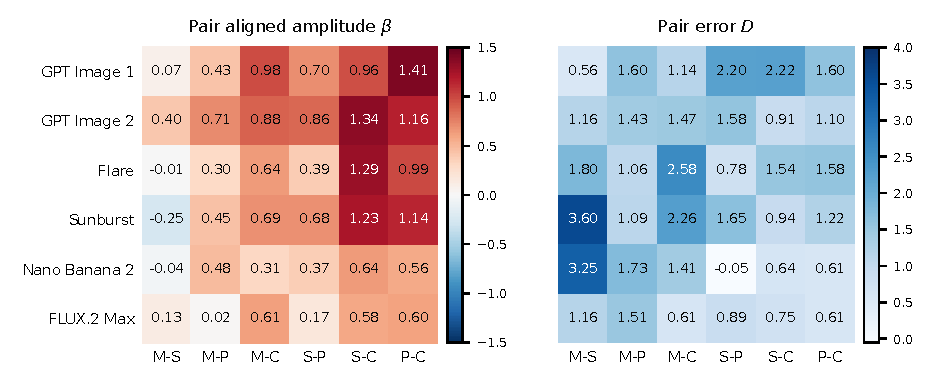
\includegraphics[width=\linewidth]{fig_pairs.pdf}
\caption{Aligned amplitude and error for each of the six painter pairs (M: Monet, S: Sisley,
P: Pissarro, C: C\'ezanne), using all 31 features and normalized by the squared reference
distance of each pair. An amplitude of 1 matches the reference, negative values point the
opposite way, and an error of 1 corresponds to no distinction. Negative errors can arise from
repeat correction.}
\label{fig:pairs}
\end{figure}

\paragraph{Full decomposition.} Table~\ref{tab:decomposition-full} gives all components; against the
artist-free baseline the shared component is $N_{\mathrm{free}}=G+N+I$, with $G$ the squared
generic-minus-free shift and $I$ a signed cross term (Appendix~\ref{app:estimators}). Against
the artist-free baseline, 82.5--95.7\% of the squared change is shared; this includes the
painting instruction itself, and computing both components within scenes gives 88.6--97.2\%.
Against the generic baseline the within-scene shares are 52.8--93.6\%. Table~\ref{tab:robustness}
reports centroid proximity in squared standardized units.

\paragraph{Feature families.} Table~\ref{tab:families} gives the shared fraction by family, with the
mean faithful and exact-differences values. The faithful benchmark is higher for texture than for
color (+2.1 points), the exact-differences benchmark lower ($-$3.2 points; both computed before
rounding), so neither benchmark explains the texture--color difference alone. Reweighting the 31
features gives shared fractions of 66.1--89.8\% (equal family weights) and 65.8--86.9\%
(development covariance), and deleting any single feature keeps the fraction within 64.8--89.6\%. Scene resamples in
which a family's denominator was not positive were dropped: 32 of 5,000 for the spatial and 4 for
the texture mean, and 35 for the paired family differences.

\paragraph{Genuine-painting controls.} For each of 1,000 random splits, the works in each
painter's collection (or each painter and content class) are divided into two disjoint halves;
the smaller half estimates the target, and the other supplies two distinct works per painter for
each of 14 pseudo-scenes (11 with content classes), which are scored with the same error $D$ in
each representation (Table~\ref{tab:genuine}). An earlier version of this control drew the two
works with replacement, so that both pseudo-repeats could be the same painting; the product of a
work with itself adds its within-painter variance, which inflated that version's means (0.234,
0.753 and 0.731, first column). With distinct works the pseudo-repeats are unbiased for the
painter's mean, so the pooled control's expected value is the noise of the target alone: for a
target estimated from about half of each collection, the term $\frac34\sum_a\operatorname{tr}
(\Sigma_a)/n_a$ of Appendix~\ref{app:estimators} is about twice the 6.7\% of $H$ found for the full
collections, close to the observed 0.125. Content-class sampling adds the difference between class
and pooled means (0.185), and class-specific targets rest on fewer works (0.328). The generated
errors are scored against the full collections, whose target noise is the 6.7\% removed by the
correction of $H$ (Table~\ref{tab:robustness}). These controls therefore describe what genuine
paintings score under this design; they do not bound what a generator could reach.

\paragraph{Feature separability.} Classifying each of the 221 development works by its nearest
reference mean in the 31 standardized features gives 49.8\% macro accuracy, with 39.6\% of Monet
and 30.6\% of Sisley works correct; the embeddings give 79.8\% (CLIP) and 79.6\% (CSD).

\paragraph{Painter pairs and coverage.} Table~\ref{tab:coverage} shows that the aggregate
aligned response rests mostly on the first reference component, which accounts for 66.3\% of
the reference spread, and that omitting C\'ezanne removes much of it. Stronger pair alignment
does not ensure lower pair error: GPT Image 1 has weaker Monet--Sisley alignment than GPT Image
2 but lower error for that pair (Figure~\ref{fig:pairs}). For Flare, Sunburst and Nano Banana
2, swapping the Monet and Sisley reference labels lowers the overall error, as it must when the
pair alignment is negative.

\paragraph{Scene aggregation and rescaling.} Nano Banana 2 has the largest scene variation and
FLUX.2 Max the smallest, which explains their reversal between $D$ and $D_{\mathrm{agg}}$. GPT
Image 2's differences are about twice the reference size in squared size (1.49 times in norm), so
shrinking them to about 0.45 of their size removes more off-pattern difference than aligned
response. Deleting any scene and
refitting the whole procedure preserves GPT Image 2's advantage after rescaling.

\paragraph{Distributions.} Table~\ref{tab:diversity} gives the prespecified distribution
diagnostics. The 28 images named for a painter span 14 scenes, yet their total variance is 0.25--0.88
of that of the painter's reference works. The named images are closer than the generic images to the
painter's works in energy distance in 21 of 24 configuration--painter combinations.
Figure~\ref{fig:projection} shows each configuration's scene-averaged centered named means next to
the reference differences on the first two reference axes, which carry 87.0\% of $H$.

% Generated by paper/tmlr/build_assets.py; do not edit by hand.
% input data/manifests/painter_specificity_v2/psv2-20260911/analysis.json sha256 c1d21b16f840a10fd253c1d558743a09671acf3d4e48601ddcc96625a5a90be0
\begin{table}[t]
\caption{Prespecified distribution diagnostics in the 31 features. Trace ratio: total variance of the 28 images named for a painter (14 scenes, two repeats) relative to that of the painter's reference works. Energy distance: between those images and the painter's reference works, averaged over painters, for the named and for the generic images; named closer: number of painters (of four) for which the named images are closer.}
\label{tab:diversity}
\vspace{2pt}
\centering\small
\begin{tabular}{@{}lrrrrrrr@{}}
\toprule
 & \multicolumn{4}{c}{Trace ratio} & \multicolumn{3}{c}{Energy distance}\\
\cmidrule(lr){2-5}\cmidrule(l){6-8}
Configuration & Mon. & Sis. & Pis. & C\'ez. & named & generic & named closer\\
\midrule
GPT Image 1 & 0.48 & 0.69 & 0.60 & 0.60 & 2.64 & 4.94 & 4\\
GPT Image 2 & 0.28 & 0.31 & 0.30 & 0.30 & 2.20 & 2.76 & 4\\
Flare & 0.27 & 0.37 & 0.32 & 0.27 & 2.11 & 2.01 & 2\\
Sunburst & 0.25 & 0.27 & 0.27 & 0.32 & 1.81 & 2.36 & 3\\
Nano Banana 2 & 0.83 & 0.71 & 0.57 & 0.88 & 2.50 & 3.43 & 4\\
FLUX.2 Max & 0.34 & 0.42 & 0.57 & 0.62 & 1.35 & 2.37 & 4\\
\bottomrule
\end{tabular}
\end{table}


\begin{figure}[ht]
\centering
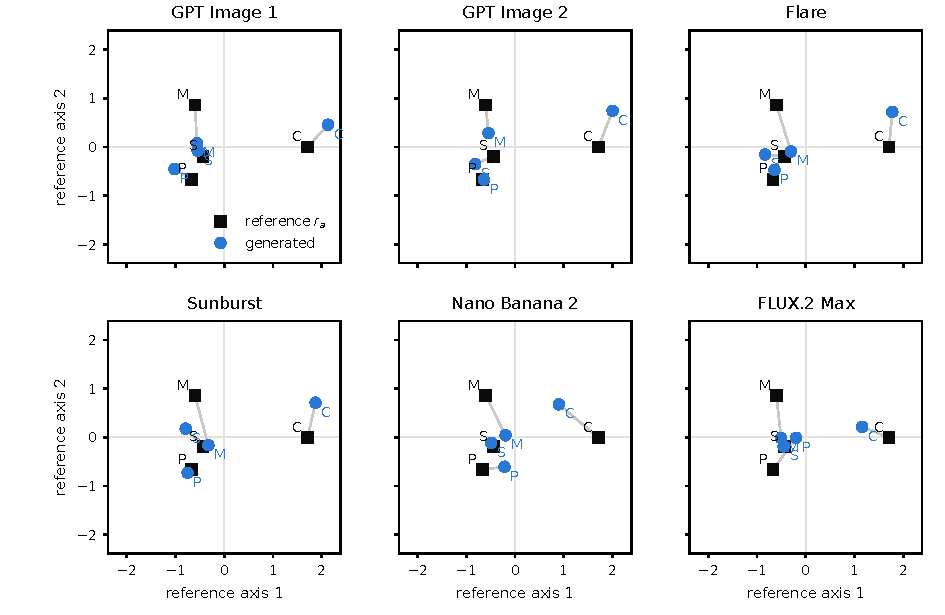
\includegraphics[width=\linewidth]{fig_projection.pdf}
\caption{Reference differences $r_a$ (squares) and each configuration's scene- and
repeat-averaged centered named means (circles) on the first two principal axes of the 31-feature
reference differences (M: Monet, S: Sisley, P: Pissarro, C: C\'ezanne; gray lines join each
painter's two points). Point values; the remaining axes are not shown.}
\label{fig:projection}
\end{figure}

\paragraph{Reference sensitivity.} The content-matched target uses the title-derived water,
built and land classes for the 11 non-mixed scenes; works in the route class enter the pooled
target but no class target, because no scene belongs to that class. The source audit recorded removable
frames, margins, labels and calibration strips; 43 uncertain boundaries were left unchanged. A
visual content audit of the same reproductions disagreed with the title-derived class for 230
works; replacing the title-derived with visual labels also leaves FLUX.2 Max with the lowest
error. All works and features are retained under every correction.

\FloatBarrier
\section{Feature families and sensitivity}\label{app:sensitivity}

\paragraph{Feature families.} Averaged over configurations, the shared fraction is 74.3\% in color,
71.5\% in spatial and 68.2\% in texture features, but the exact-differences benchmark is also lower
for texture (74.7\%, against 77.8\% for color and 79.1\% for spatial), and every family lies 3.6--7.6
points below its benchmark (Table~\ref{tab:families}). The texture--color difference of
$-$6.1 points [$-$13.5, $-$2.0] is therefore partly expected from the reference differences, and the
texture--spatial ordering is not resolved (texture lower in 65.2\% of paired scene resamples). GPT
Image 1's texture fraction, 48.6\%, the only value below 50\%, comes from oversized texture
differences ($B/H=$ 3.11; exact-differences value 74.6\%). An earlier collection of 2,000 SD-Turbo
images with a different template and seed design shares 64.2\% of the change across all features
and 36.6\% in texture, against faithful and exact-differences values of 92.5\% and 67.4\% overall
(Appendix~\ref{app:sdturbo}); it reuses the references and serves as a retrospective check.

\paragraph{Reference sources.} The shared fraction does not depend on the reference collection; its
benchmarks and the agreement scores do. AI assistants audited all 870 reference and development
reproductions and cropped peripheral artifacts such as frames and calibration strips from 131 of
them; the crops were not verified by a human. With the cropped regions and the original feature
scaling, FLUX.2 Max's error becomes 0.832, all six aligned amplitudes remain above zero, and of the
pairwise differences only Flare--FLUX.2 Max remains resolved. After also refitting the feature
scaling, FLUX.2 Max's error is 0.872, the amplitudes remain above zero, and Flare--FLUX.2 Max and GPT
Image 1--FLUX.2 Max are resolved.

\paragraph{Other checks.} FLUX.2 Max keeps the lowest 31-feature error estimate under every
single-scene deletion, square measurement windows, content-matched reference targets, both
alternative feature weightings and both source corrections (Table~\ref{tab:sensitivity}),
but in texture features alone Nano Banana 2 is lower, 0.886 against 0.906 (Appendix
Table~\ref{tab:family-agreement}). Correcting the reference spread $H$ for its finite-sample bias
(6.7\%) scales $\beta$, $Q$ and $D-1$ by the same factor: the aligned amplitudes become
0.474--1.071, FLUX.2 Max's error 0.787, no ordering changes, and the exact-differences fractions
rise to 59.3--85.1\% (Table~\ref{tab:robustness}). The named images of every configuration
are less varied than the painter's reference works (trace ratios 0.25--0.88), and they are closer
to the painter's works than the generic images in 21 of 24 configuration--painter combinations
(Table~\ref{tab:diversity}).

\FloatBarrier
\section{Learned embeddings}\label{app:learned}

\paragraph{Extraction.} We used the public checkpoints
\texttt{openai/\allowbreak clip-\allowbreak vit-\allowbreak large-\allowbreak patch14} and
\texttt{tomg-\allowbreak group-\allowbreak umd/\allowbreak CSD-\allowbreak ViT-\allowbreak L}. CSD uses its released style projection of the CLIP visual
backbone; its release notes a discrepancy with the published benchmark numbers, so we
characterize the released checkpoint without claiming to reproduce those numbers. Every image
is orientation- and color-corrected as above, resized bicubically to a 224-pixel short side,
center-cropped to $224\times224$ and normalized with the CLIP channel statistics. Embeddings
are unit-normalized 768-dimensional vectors; we use their Euclidean and cosine geometry without
scaling or dimension selection. Backend and batch-size checks on fixed test cases agreed to
within $1.3\times10^{-6}$ per coordinate.

\paragraph{Prototype gain.} With unnormalized prototypes $\mu_a$ (means of unit reference
embeddings), $g_a^\top\mu_b$ is the average image-to-reference cosine similarity. Writing
$g_a=\bar g+d_a$ and $\mu_a=\bar\mu+r_a$,
\begin{equation}
\frac14\sum_a g_a^\top\mu_a-g_{\mathrm g}^\top\bar\mu
=(\bar g-g_{\mathrm g})^\top\bar\mu+\frac14\sum_a d_a^\top r_a
=(\bar g-g_{\mathrm g})^\top\bar\mu+\frac{H\widehat\beta}{4},
\end{equation}
because $\sum_a r_a=\sum_a d_a=0$. The first term cannot depend on which name produced which
images; permuting the painter labels of the generated images changes only $\widehat\beta$. The
faithful value sets $g_a=\mu_a$, giving the shared fraction $(\bar\mu-g_{\mathrm
g})^\top\bar\mu/[(\bar\mu-g_{\mathrm g})^\top\bar\mu+H/4]$. Replacing $\mu_a$ by the unit
prototype $u_a=\mu_a/\|\mu_a\|$ keeps the score linear in the image embedding, so the same
identity holds with $u_a$ in place of $\mu_a$ (Table~\ref{tab:learned-settings}).

% Generated by paper/tmlr/build_assets.py; do not edit by hand.
% input reports/painter_tmlr_diagnostics_v1/analysis.json sha256 76792fa35f90e3d8fec1a75b0eec27d69cac14ed875fce8b64096b8e2525a4d4
% input reports/painter_tmlr_diagnostics_v5/analysis.json sha256 5747902e4fae5ff111a52b5f2b8da112bc26c611555e82314b278de953981f6b
\begin{table}[t]
\caption{Which configuration is best on each readout when the 14 scenes are resampled with replacement (5,000 paired resamples; the same scenes for every configuration). The percentages describe dependence on the authored scenes. Ties, which occur for recognition, are credited to the configuration listed first. Lower rows: alignment ratio and $D_{\mathrm{held}}$ (separate resamples).}
\label{tab:stability}
\vspace{2pt}
\centering\small
\begin{tabular}{@{}llrlr@{}}
\toprule
Readout & Most often best & \% & Next & \%\\
\midrule
Proximity gain, CLIP & Nano Banana 2 & 85.8 & Sunburst & 9.5\\
Proximity gain, CSD & FLUX.2 Max & 33.6 & GPT Image 1 & 26.2\\
Recognition, CLIP & GPT Image 2 & 98.7 & GPT Image 1 & 0.8\\
Recognition, CSD & GPT Image 2 & 80.4 & GPT Image 1 & 19.6\\
Error $D$, 31 features & FLUX.2 Max & 84.7 & Nano Banana 2 & 15.3\\
Error $D$, CLIP & GPT Image 1 & 99.3 & GPT Image 2 & 0.6\\
Error $D$, CSD & FLUX.2 Max & 47.2 & GPT Image 1 & 26.8\\
\midrule
Alignment ratio, 31 features & GPT Image 2 & 98.0 & Nano Banana 2 & 0.7\\
Alignment ratio, CLIP & GPT Image 2 & 99.7 & GPT Image 1 & 0.3\\
Alignment ratio, CSD & GPT Image 2 & 100.0 & FLUX.2 Max & 0.0\\
$D_{\mathrm{held}}$, 31 features & GPT Image 2 & 99.0 & GPT Image 1 & 0.6\\
$D_{\mathrm{held}}$, CLIP & GPT Image 2 & 99.8 & GPT Image 1 & 0.2\\
$D_{\mathrm{held}}$, CSD & GPT Image 2 & 100.0 & FLUX.2 Max & 0.0\\
\bottomrule
\end{tabular}
\end{table}

% Generated by paper/tmlr/build_assets.py; do not edit by hand.
% input reports/painter_learned_audit_v1/analysis.json sha256 06c77de4be133afc203dda122b2816d4f866e1389999f18bc94b3d9c668f28f7
% input reports/painter_tmlr_diagnostics_v3/analysis.json sha256 2aa36a87cd6d23ee909cdf94bd9f512d5743138f1d8a8f7c236d56f33fbceb57
\begin{table}[t]
\caption{Share (\%) of the proximity gain supplied by the shared term under alternative reference settings. Prim.: full reproductions of the primary reference collection (Table~\ref{tab:learned}). Crop: reference reproductions replaced by their audited painting regions. Dev.: the development panel as the reference target. Both: audited regions of the development panel. Unit: primary prototypes normalized to unit length, as in recognition.}
\label{tab:learned-settings}
\vspace{2pt}
\centering\small\setlength{\tabcolsep}{3.5pt}
\begin{tabular}{@{}lrrrrrrrrrr@{}}
\toprule
 & \multicolumn{5}{c}{CLIP} & \multicolumn{5}{c}{CSD}\\
\cmidrule(lr){2-6}\cmidrule(l){7-11}
Configuration & prim. & crop & dev. & both & unit & prim. & crop & dev. & both & unit\\
\midrule
GPT Image 1 & 74.5 & 74.5 & 74.3 & 74.4 & 74.6 & 72.7 & 72.9 & 73.4 & 73.0 & 72.8\\
GPT Image 2 & 73.2 & 73.0 & 72.8 & 72.7 & 73.4 & 54.2 & 54.7 & 53.5 & 53.2 & 54.7\\
Flare & 78.8 & 78.7 & 78.9 & 79.0 & 79.0 & 65.0 & 65.5 & 65.1 & 64.9 & 65.4\\
Sunburst & 77.7 & 77.7 & 78.0 & 78.1 & 78.0 & 67.4 & 67.6 & 68.0 & 67.8 & 67.7\\
Nano Banana 2 & 83.8 & 83.9 & 83.5 & 83.7 & 83.9 & 79.7 & 79.9 & 81.3 & 81.0 & 79.6\\
FLUX.2 Max & 81.7 & 81.7 & 81.5 & 81.9 & 81.9 & 77.6 & 77.7 & 78.7 & 78.5 & 77.7\\
\bottomrule
\end{tabular}
\end{table}

% Generated by paper/tmlr/build_assets.py; do not edit by hand.
% input reports/painter_tmlr_diagnostics_v5/analysis.json sha256 5747902e4fae5ff111a52b5f2b8da112bc26c611555e82314b278de953981f6b
\begin{table}[t]
\caption{Error parts and repeat dependence in each representation. $\beta$: unadjusted paired-scene Student 95\% intervals. Split of $D$: the prespecified parts along and off the reference pattern (Table~\ref{tab:calibration}) and the off-pattern share. Repeat noise: half the squared difference between the repeats' centered contrasts, relative to $H$. $\rho$ at $D=1$: common repeat correlation at which an error above 1 would fall to 1 if the repeats shared that fraction of their noise (Appendix~\ref{app:provenance}); errors below 1 would only fall further.}
\label{tab:embedding-calibration}
\vspace{2pt}
\centering\small\setlength{\tabcolsep}{4pt}
\begin{tabular}{@{}lcrrrrrr@{}}
\toprule
 & $\beta$ & & \multicolumn{3}{c}{Split of $D$} & Repeat &\\
\cmidrule(lr){4-6}
Configuration & scenes & $D$ & along & off-pattern & off (\%) & noise $/H$ & $\rho$ at $D=1$\\
\midrule
\multicolumn{8}{@{}l}{\textit{31 features}}\\
GPT Image 1 & [0.806, 1.070] & 1.572 & 0.029 & 1.543 & 98.2 & 2.02 & 0.22\\
GPT Image 2 & [0.938, 1.059] & 1.226 & $-$0.003 & 1.229 & 100.2 & 0.96 & 0.19\\
Flare & [0.719, 0.824] & 1.738 & 0.054 & 1.683 & 96.9 & 0.42 & 0.64\\
Sunburst & [0.741, 0.907] & 1.641 & 0.044 & 1.598 & 97.3 & 0.58 & 0.52\\
Nano Banana 2 & [0.335, 0.549] & 1.109 & 0.317 & 0.793 & 71.5 & 2.60 & 0.04\\
FLUX.2 Max & [0.337, 0.603] & 0.801 & 0.304 & 0.497 & 62.0 & 1.67 & ---\\
\midrule
\multicolumn{8}{@{}l}{\textit{CLIP}}\\
GPT Image 1 & [0.468, 0.585] & 0.847 & 0.231 & 0.616 & 72.8 & 1.20 & ---\\
GPT Image 2 & [0.716, 0.825] & 1.061 & 0.057 & 1.004 & 94.6 & 1.13 & 0.05\\
Flare & [0.511, 0.606] & 1.057 & 0.201 & 0.856 & 81.0 & 0.80 & 0.07\\
Sunburst & [0.594, 0.709] & 1.136 & 0.129 & 1.007 & 88.6 & 0.83 & 0.14\\
Nano Banana 2 & [0.472, 0.574] & 1.078 & 0.230 & 0.848 & 78.7 & 1.59 & 0.05\\
FLUX.2 Max & [0.385, 0.490] & 1.058 & 0.316 & 0.743 & 70.2 & 1.78 & 0.03\\
\midrule
\multicolumn{8}{@{}l}{\textit{CSD}}\\
GPT Image 1 & [0.654, 0.803] & 0.735 & 0.085 & 0.650 & 88.4 & 0.73 & ---\\
GPT Image 2 & [0.889, 0.982] & 0.741 & 0.005 & 0.736 & 99.4 & 0.54 & ---\\
Flare & [0.768, 0.841] & 0.819 & 0.041 & 0.778 & 95.0 & 0.36 & ---\\
Sunburst & [0.813, 0.906] & 0.944 & 0.024 & 0.920 & 97.4 & 0.42 & ---\\
Nano Banana 2 & [0.463, 0.588] & 0.999 & 0.231 & 0.768 & 76.9 & 1.04 & ---\\
FLUX.2 Max & [0.540, 0.656] & 0.714 & 0.162 & 0.551 & 77.3 & 1.01 & ---\\
\bottomrule
\end{tabular}
\end{table}

% Generated by paper/tmlr/build_assets.py; do not edit by hand.
% input reports/painter_tmlr_diagnostics_v1/analysis.json sha256 76792fa35f90e3d8fec1a75b0eec27d69cac14ed875fce8b64096b8e2525a4d4
\begin{table}[t]
\caption{Shared fraction $N/(N+B)$ (\%) of the squared change added by the names, computed in each embedding, with its faithful-imitation value.}
\label{tab:learned-squared}
\vspace{2pt}
\centering\small
\begin{tabular}{@{}lrrrr@{}}
\toprule
 & \multicolumn{2}{c}{CLIP} & \multicolumn{2}{c}{CSD}\\
\cmidrule(lr){2-3}\cmidrule(l){4-5}
Configuration & observed & faithful & observed & faithful\\
\midrule
GPT Image 1 & 76.1 & 86.1 & 76.5 & 89.2\\
GPT Image 2 & 76.6 & 87.1 & 68.8 & 82.4\\
Flare & 81.7 & 88.7 & 74.6 & 86.4\\
Sunburst & 77.6 & 88.9 & 69.9 & 86.9\\
Nano Banana 2 & 82.3 & 91.2 & 77.4 & 89.7\\
FLUX.2 Max & 80.8 & 88.5 & 75.1 & 87.7\\
\bottomrule
\end{tabular}
\end{table}

% Generated by paper/tmlr/build_assets.py; do not edit by hand.
% input reports/painter_tmlr_diagnostics_v2/analysis.json sha256 bed891f767a98f4b281b6783b1021956f4d2c3ff80becbf6b2693ee45987ef1a
\begin{table}[t]
\caption{Shared part (\%) of the proximity gain for each prompted painter separately: $(\bar g-g_{\mathrm g})^\top\mu_a$ divided by $(g_a-g_{\mathrm g})^\top\mu_a$. Values above 100\% mean that the painter-specific term is negative for that painter.}
\label{tab:per-painter}
\vspace{2pt}
\centering\small\setlength{\tabcolsep}{4pt}
\begin{tabular}{@{}lrrrrrrrr@{}}
\toprule
 & \multicolumn{4}{c}{CLIP} & \multicolumn{4}{c}{CSD}\\
\cmidrule(lr){2-5}\cmidrule(l){6-9}
Configuration & Mon. & Sis. & Pis. & C\'ez. & Mon. & Sis. & Pis. & C\'ez.\\
\midrule
GPT Image 1 & 75.4 & 85.7 & 81.2 & 59.5 & 73.8 & 79.6 & 73.1 & 62.0\\
GPT Image 2 & 78.1 & 85.5 & 91.9 & 51.6 & 68.8 & 62.1 & 64.1 & 34.6\\
Flare & 84.7 & 93.3 & 102.9 & 55.1 & 74.1 & 68.1 & 85.8 & 47.5\\
Sunburst & 90.2 & 83.7 & 93.5 & 57.2 & 75.3 & 70.4 & 78.4 & 53.4\\
Nano Banana 2 & 87.6 & 90.0 & 87.6 & 73.2 & 79.1 & 79.1 & 73.4 & 85.8\\
FLUX.2 Max & 80.5 & 105.3 & 97.0 & 57.6 & 70.6 & 86.4 & 96.9 & 64.0\\
\bottomrule
\end{tabular}
\end{table}


\paragraph{Error parts and repeat dependence.} Table~\ref{tab:embedding-calibration} gives the split
of $D$, Student intervals for $\beta$ and the repeat noise in all three representations. In the
embeddings the off-pattern part also dominates, and the amplitude along the pattern contributes
more than in the features.

\paragraph{Crops.} Generated images are square, so the encoders' center crop sees nearly the whole
image, whereas non-square reference reproductions lose their periphery. For the 31 features the
comparable square-window sensitivity leaves FLUX.2 Max with the lowest error (Appendix
Table~\ref{tab:sensitivity}).

\paragraph{Scope.} CSD is built on the CLIP backbone and both encoders see the same images, so
their agreement is weaker evidence than agreement between independent representations would be. All
four painters appear in CSD's style-tag vocabulary, and the overlap between either encoder's
training data and our references is unknown. As a check on the reference panels, the primary
prototypes classify the 221 development works with 79.8\% (CLIP) and 79.6\% (CSD) macro
accuracy.

\FloatBarrier
\section{Held-scene prompt-name recognition}\label{app:transfer}

% Generated by paper/tmlr/build_assets.py; do not edit by hand.
% input reports/painter_prototype_transfer_v1/analysis.json sha256 e1d1fbb924feb797f67e0907677511ed7c745335a4f2827e99d2f286e6be5448
\begin{table}[t]
\caption{Held-scene recognition of the prompted painter (\%, 112 named images per configuration, chance 25\%). Ref.: nearest reference prototype. Shift: the same after adding one fixed translation that aligns the generated and reference mixture means, fitted on the other 13 scenes without painter labels. Gen.: nearest generated-image prototype fitted with painter labels on the other 13 scenes. Shift and Gen.\ use more information than Ref., and Gen.\ more than Shift.}
\label{tab:transfer}
\vspace{2pt}
\centering\small
\begin{tabular}{@{}lrrrrrr@{}}
\toprule
 & \multicolumn{3}{c}{CLIP} & \multicolumn{3}{c}{CSD}\\
\cmidrule(lr){2-4}\cmidrule(l){5-7}
Configuration & Ref. & Shift & Gen. & Ref. & Shift & Gen.\\
\midrule
GPT Image 1 & 60.7 & 55.4 & 80.4 & 72.3 & 73.2 & 84.8\\
GPT Image 2 & 68.8 & 66.1 & 75.0 & 75.9 & 76.8 & 94.6\\
Flare & 59.8 & 59.8 & 77.7 & 62.5 & 74.1 & 92.9\\
Sunburst & 58.9 & 62.5 & 69.6 & 61.6 & 70.5 & 90.2\\
Nano Banana 2 & 51.8 & 59.8 & 63.4 & 50.9 & 61.6 & 75.0\\
FLUX.2 Max & 41.1 & 53.6 & 71.4 & 39.3 & 66.1 & 75.0\\
\midrule
Mean change vs.\ Ref.\ (pp) & & +2.7 & +16.1 & & +10.0 & +25.0\\
\bottomrule
\end{tabular}
\end{table}


For each configuration and held-out scene $s$, let $x$ be a unit embedding of a named image
from scene $s$ and $u_a=\mu_a/\|\mu_a\|$ the normalized reference prototypes. The reference rule
(Ref.) is $\arg\max_a x^\top u_a$. The shift rule computes $t_{-s}=\frac14\sum_a\mu_a-\bar
g_{-s}$, where $\bar g_{-s}$ is the mean of the 104 named embeddings from the other 13 scenes,
and predicts $\arg\max_a(x+t_{-s})^\top u_a$. The translation adds $t_{-s}^\top u_a$ to painter
$a$'s score; these shifts differ between painters, which is why recognition can change. Because the
same vector is added to every named image, the centered contrasts $d_{sak}$, and hence $\beta$, $Q$
and $D$, are unchanged. The generated-prototype rule (Gen.) uses the normalized mean of the 26
labeled training embeddings for each painter. Held-scene repeats never enter the fit, and the
artist-free and generic images are not used. The question was chosen after the reference-rule
confusions were known; the rules were fixed before the translated outcomes were computed. Folds
overlap and scenes are authored, so these are descriptive out-of-fold results. The mean changes
from the reference rule are +2.7 (CLIP) and +10.0 points (CSD) for the shift rule; for FLUX.2 Max in
CSD the shift corrects 39 and harms 9 of 112 decisions. The generated-prototype rule outperforms
both reference-based rules in all 12 configuration--encoder combinations, so the prompted names
are more separable within each generator's own outputs than with respect to the historical
references. Across the four
combinations of reference source (full reproductions or audited painting regions) and reference
target (primary collection or development panel), the mean translation gains are 2.2--4.0 points
(CLIP) and 9.7--10.1 points (CSD).

\FloatBarrier
\section{The SD-Turbo collection}\label{app:sdturbo}

The collection was generated on 5 September 2026 with \texttt{stabilityai/sd-turbo} at
$512\times512$ pixels, one denoising step and guidance scale zero, for an earlier, unpublished
distance analysis by the same project. It crosses 16 scenes, 25 repeat blocks and five
conditions (the baseline and four names), 400 images per condition. Within each scene and
block, all five conditions use the same seed. Its image hashes are disjoint from the main
collection, and its 16 scene descriptions are shorter, class-level texts, different from the 14
main descriptions (for example, ``a riverbank landscape, with water organizing the
composition''), and the baseline prompt already requests an oil painting, with the names inserted
as ``by [painter]''.

For block vectors $v_b$, $b=1,\dots,K$ with $K=25$, the estimator
$U(v)=[K(K-1)]^{-1}\sum_{b\ne b'}\ip{v_b}{v_{b'}}$ replaces the two-repeat product. Averaging
scenes within each block, let $\delta_{ba}$ be the named-minus-baseline shift, $c_b$ its mean
over names and $e_{ba}=\delta_{ba}-c_b$. The shared component is $4U(c)$ and the between-name
component is $\sum_aU(e_a)$. Because products are formed only between different blocks,
correlation among the five seed-matched conditions within a block is allowed. The reference
means and scaling are those of the main experiment. Deleting each block once gives the reported
ranges, which describe sensitivity to single blocks. The faithful and exact-differences benchmarks use
the block means of the baseline arm and the same cross-block products. Table~\ref{tab:sdturbo}
gives the values by feature family. Across all features the shared fraction is 64.2\%
(63.9--64.6\% across block deletions), 57.5\% in color and 84.9\% in spatial features but 36.6\%
in texture (36.2--36.9\%); within scenes it is 72.4\% overall and 48.5\% for texture. The
exact-differences value in texture is 46.5\%. SD-Turbo's aligned amplitude is 0.618, its
scene-averaged error 0.917 and its scene-wise error 1.637, and its Monet--Sisley alignment is
0.471. The collection reuses the same references and was analyzed before in other ways.

% Generated by paper/tmlr/build_assets.py; do not edit by hand.
% input reports/painter_cross_cohort_v1/analysis.json sha256 9488dfafa5779b8b065cc756804e67ad64c2841a5c62c2f9b0105f8fef13973e
% input reports/painter_tmlr_diagnostics_v2/analysis.json sha256 bed891f767a98f4b281b6783b1021956f4d2c3ff80becbf6b2693ee45987ef1a
\begin{table}[t]
\caption{Shared fraction (\%) in the SD-Turbo collection by feature family: pooled over scenes, its range over the 25 single-block deletions, computed within scenes, and the faithful and exact-differences benchmarks.}
\label{tab:sdturbo}
\vspace{2pt}
\centering\small
\begin{tabular}{@{}lrcrrr@{}}
\toprule
Features & shared (\%) & block deletions & within scene & faithful & exact diff.\\
\midrule
All 31 & 64.2 & 63.9--64.6 & 72.4 & 92.5 & 67.4\\
Color (11) & 57.5 & 57.3--57.8 & 66.6 & 79.7 & 56.4\\
Spatial (8) & 84.9 & 84.4--85.3 & 81.2 & 96.8 & 83.3\\
Texture (12) & 36.6 & 36.2--36.9 & 48.5 & 89.8 & 46.5\\
\bottomrule
\end{tabular}
\end{table}


\FloatBarrier
\section{The second collection}\label{app:second}

\paragraph{Protocol and amendments.} After the four-painter results were known, a protocol for a
second collection named the two further groups, fixed the tests H1 and H2
(Section~\ref{sec:inference}) and the per-group analysis, and was frozen with the request frame
before any image was generated. The freeze record binds the hashes of the protocol file and of the
analysis code as approved, so the protocol's header still reads ``draft''; the correction of H2 for
panel size is in that frozen code. The plan for the embedding readouts (shared-fraction intervals,
recognition and proximity) was fixed while the images were being collected and before any was
measured. The reference rules were amended twice before the first request. First, the protocol's
minimum of 60 works per painter was withdrawn so that the new collections are treated exactly like
the four-painter collection, which had none; three Hudson River painters and Kirchner fall below it
(Table~\ref{tab:v3-panels}). Second, Wikimedia Commons now serves only standard thumbnail widths,
so the rendered files are 1,280, 1,920 or 3,840 pixels wide (or the original), all reduced to a
512-pixel short side for measurement. The title lexicon keeps every term of the four-painter
lexicon and adds place and landscape terms for the new painters' titles (for example Yosemite,
Catskill, piazza and wheatfield) and exclusion terms for figure and interior titles that those
words would otherwise admit; the terms were fixed from the titles before any image was requested.
A first proposal for the related group, four Russian landscape painters, was replaced before any
reference was acquired, because Wikidata records too few documented oil paintings for three of them.

% Generated by paper/tmlr/build_assets.py; do not edit by hand.
% input data/manifests/painter_specificity_v3/refs-20261002/determination_receipt.json sha256 39e289f1ba44c7d5fe8ae18d59d076a07eb1cefd6d105859b3565bb6576fa982
% input data/manifests/painter_specificity_v3/refs-20261002/measurement_receipt.json sha256 debf37377410a96cd64f1714a277ade667d959714c0c13bbd7af986de0795c16
\begin{table}[t]
\caption{Reference panels of the two further painter groups: Wikidata paintings with a Commons image, and how many remain after each gate, applied in order as for the four-painter panel (single creator, oil on canvas, a collection, an open licence, a short side of at least 1,024 pixels, an outdoor title); then works measured after merging duplicates and excluding unreadable files. Classes are water/built/route/land by title.}
\label{tab:v3-panels}
\vspace{2pt}
\centering\footnotesize
\begin{tabular}{lrrrrrrrrr}
\toprule
Painter & Found & Creator & Medium & Coll. & Rights & Size & Title & Measured & W/B/R/L \\
\midrule
\multicolumn{10}{l}{\emph{Century group}} \\
van Ruisdael & 485 & 470 & 261 & 219 & 218 & 127 & 123 & 123 & 58/31/3/31 \\
Canaletto & 408 & 404 & 342 & 306 & 306 & 166 & 158 & 157 & 120/37/0/1 \\
van Gogh & 887 & 887 & 818 & 638 & 638 & 587 & 255 & 255 & 25/95/12/123 \\
Kirchner & 273 & 273 & 207 & 190 & 187 & 153 & 43 & 41 & 10/17/2/14 \\
\multicolumn{10}{l}{\emph{Hudson River School}} \\
Bierstadt & 481 & 481 & 228 & 138 & 138 & 103 & 92 & 92 & 36/5/0/51 \\
Church & 153 & 152 & 101 & 81 & 81 & 51 & 47 & 47 & 11/3/0/33 \\
Cole & 172 & 172 & 108 & 99 & 99 & 63 & 36 & 36 & 7/7/0/22 \\
Durand & 204 & 204 & 183 & 163 & 163 & 57 & 38 & 37 & 9/2/1/26 \\
\bottomrule
\end{tabular}
\end{table}


\paragraph{References and predictions.} Of 790 works admitted after merging two duplicates, one
file in an unsupported format could not be read and one in an unprofiled non-RGB color space could
not be measured, as for the four-painter collection, leaving 788 (Table~\ref{tab:v3-panels}). The
predictions recorded before collection (Table~\ref{tab:v3-predictions}) use the first collection's
generic outputs; the four-painter rows reproduce this paper's values. The CLIP and CSD checkpoints,
deleted after the first collection's extraction, were downloaded again at the same revisions and
matched their recorded hashes.

% Generated by paper/tmlr/build_assets.py; do not edit by hand.
% input data/manifests/painter_specificity_v3/refs-20261002/predictions.json sha256 65a12c297f2f2e0c2d6d7afbb313e590bf7360001cbe82c5edc5fed20040414f
\begin{table}[t]
\caption{Predictions recorded before the second collection: the reference spread $H$ of each group and the faithful benchmark $N^*/(N^*+H)$ over the six configurations, with September's generic outputs. The four-painter rows reproduce the paper's values.}
\label{tab:v3-predictions}
\vspace{2pt}
\centering\small
\begin{tabular}{lrrrrrr}
\toprule
& \multicolumn{2}{c}{31 features} & \multicolumn{2}{c}{CLIP} & \multicolumn{2}{c}{CSD} \\
\cmidrule(lr){2-3}\cmidrule(lr){4-5}\cmidrule(lr){6-7}
Group & $H$ & faithful (\%) & $H$ & faithful (\%) & $H$ & faithful (\%) \\
\midrule
Four Impressionists & 5.92 & 84.8--95.2 & 0.139 & 86.1--91.2 & 0.325 & 82.4--89.7 \\
Century group & 34.61 & 47.0--73.3 & 0.460 & 67.4--74.8 & 1.048 & 63.4--70.3 \\
Hudson River School & 6.24 & 90.1--96.9 & 0.082 & 92.7--94.3 & 0.142 & 92.2--95.5 \\
\bottomrule
\end{tabular}
\end{table}


\paragraph{Collection.} The six configurations kept the first collection's routes and request
fields; tests in the code check that the no-clause and generic requests are identical to the first
collection's for every configuration and scene, and the gateway listed every route at unchanged
prices on the day of collection. The 1,680 requests were randomized within scene blocks of 120
with a new seed. Two requests were refused by the provider's safety system (HTTP 400, no charge)
for prompts that name Durand and Bierstadt with ordinary landscape scenes; under the protocol they
are recorded and not repeated. Two gateway timeouts (HTTP 503) were repeated successfully. The new
charges were \$72.93. The collector reserves \$5 for every request until its charge is known and
keeps that reservation when a failure reports no charge, so the two timeouts held \$10 that the
bookkeeping never released; the spending ceiling was therefore raised from \$200 to \$220 in a
recorded amendment, which changed no other rule.

% Generated by paper/tmlr/build_assets.py; do not edit by hand.
% input reports/painter_specificity_v3/analysis.json sha256 75ef2a23c04a5c570fd224a0ada396271ad7026ef0657a1908023daca709cbc4
\begin{table}[t]
\caption{The two prespecified tests in every representation (the 31 features in the full view are primary). H1: mean over configurations of the century group's shared fraction minus the Hudson River School's (percentage points), with a 95\% interval from 5,000 paired scene resamples. H2: Spearman correlation over the 28 painter pairs between the name distance and the reference distance, averaged over configurations, with the exact one-sided $p$-value over all 40,320 relabellings of the eight painters (a Mantel test, \citealp{mantel1967detection}); the reference distances are corrected for panel size, and the uncorrected test is shown beside it. In the central square window H1 is unchanged by construction, because the generated images are square and the shared fraction does not use the references. Last columns: reference spread corrected for panel size.}
\label{tab:v3-tests}
\vspace{2pt}
\centering\small\setlength{\tabcolsep}{4pt}
\begin{tabular}{@{}lrcrrrrrr@{}}
\toprule
 & \multicolumn{2}{c}{H1: century $-$ Hudson} & \multicolumn{2}{c}{H2: Mantel} & \multicolumn{2}{c}{H2, uncorrected} & \multicolumn{2}{c}{$H$, noise-corrected}\\
\cmidrule(lr){2-3}\cmidrule(lr){4-5}\cmidrule(lr){6-7}\cmidrule(l){8-9}
Representation & diff. & 95\% & $\rho$ & $p$ & $\rho$ & $p$ & century & Hudson\\
\midrule
31 features & $-$72.7 & [$-$76.5, $-$62.6] & 0.85 & $<$0.001 & 0.84 & $<$0.001 & 33.80 & 4.21\\
31 features, central square & $-$72.7 & [$-$76.5, $-$62.6] & 0.85 & 0.001 & 0.85 & 0.001 & 35.30 & 5.07\\
CLIP & $-$40.1 & [$-$41.4, $-$37.3] & 0.86 & $<$0.001 & 0.86 & $<$0.001 & 0.452 & 0.070\\
CSD & $-$47.4 & [$-$48.9, $-$44.9] & 0.92 & $<$0.001 & 0.92 & $<$0.001 & 1.034 & 0.116\\
\bottomrule
\end{tabular}
\end{table}


\paragraph{Tests and sensitivity.} H1 and H2 hold in every representation, and H2 also holds in the
central square window and without the correction for panel size (Table~\ref{tab:v3-tests}); H1 is
unchanged in the central square window by construction, because the generated images are square
and the shared fraction does not use the references. The per-configuration differences in shared
fraction are large in every configuration. For FLUX.2 Max the adjusted interval is wide because
both of its fractions are unstable under resampling: the prespecified H1 code keeps resamples whose
denominator is not positive, and for FLUX.2 Max with the Hudson River School $N+B\le0$ in 90 of the
5,000 draws, while a fraction lies outside $[0,1]$ in 150 draws for the century group and 237 for
the Hudson River School (Table~\ref{tab:v3-shared}). No other configuration has a non-positive
denominator.

\paragraph{Breakdowns defined after review.} Table~\ref{tab:v3-closeness} splits the two tests
descriptively, under a plan written after a first review of these results; the reviewers had
already computed the point values, and the intervals are new. H2 holds within the century group and
across the groups, and is weak within the Hudson River School, where the reference differences are
small and only six pairs enter. A faithful imitator would show a century-minus-Hudson difference of
30.9 points in the features, so the remaining 41.8 points come from how strongly the generators
separate the names. Table~\ref{tab:v3-readouts} adds the readouts of the embedding plan that the
main text does not quote.

% Generated by paper/tmlr/build_assets.py; do not edit by hand.
% input reports/painter_specificity_v3/analysis.json sha256 75ef2a23c04a5c570fd224a0ada396271ad7026ef0657a1908023daca709cbc4
\begin{table}[t]
\caption{Agreement of the between-name differences with each group's reference differences (31 features, second collection), as in Table~\ref{tab:agreement}: aligned amplitude $\beta$ and error $D$ with unadjusted paired-scene Student intervals, relative size $Q$, alignment ratio, held-out rescaled error, and the share of the centroid proximity gain (Eq.~\ref{eq:prototype-gain}, here in the features) carried by the shared term.}
\label{tab:v3-detail}
\vspace{2pt}
\centering\small\setlength{\tabcolsep}{4pt}
\begin{tabular}{@{}lrcrrrcrr@{}}
\toprule
Configuration & $\beta$ & 95\% & $Q$ & $\beta/\sqrt{Q}$ & $D$ & 95\% & $D_{\mathrm{held}}$ & shared gain (\%)\\
\midrule
\multicolumn{9}{l}{\emph{Century group}}\\
GPT Image 1 & 1.28 & [1.11, 1.45] & 3.13 & 0.72 & 1.58 & [0.74, 2.41] & 0.50 & 100.7\\
GPT Image 2 & 1.14 & [1.06, 1.22] & 2.22 & 0.76 & 0.94 & [0.75, 1.13] & 0.42 & 73.0\\
Flare & 1.29 & [1.21, 1.38] & 2.58 & 0.80 & 0.99 & [0.76, 1.23] & 0.35 & 76.2\\
Sunburst & 1.24 & [1.19, 1.30] & 2.61 & 0.77 & 1.12 & [0.84, 1.40] & 0.41 & 89.1\\
Nano Banana 2 & 1.04 & [0.93, 1.15] & 2.21 & 0.70 & 1.13 & [0.50, 1.77] & 0.53 & 86.2\\
FLUX.2 Max & 0.84 & [0.75, 0.93] & 1.41 & 0.71 & 0.73 & [0.60, 0.85] & 0.50 & 31.5\\
\multicolumn{9}{l}{\emph{Hudson River School}}\\
GPT Image 1 & $-$0.01 & [$-$0.12, 0.09] & 0.22 & $-$0.03 & 1.25 & [0.86, 1.64] & 1.00 & --\\
GPT Image 2 & 0.04 & [$-$0.06, 0.15] & 0.12 & 0.13 & 1.03 & [0.75, 1.31] & 1.05 & 100.2\\
Flare & $-$0.01 & [$-$0.09, 0.06] & 0.61 & $-$0.01 & 1.63 & [1.32, 1.95] & 1.00 & 103.3\\
Sunburst & 0.11 & [0.01, 0.22] & 0.48 & 0.16 & 1.26 & [1.04, 1.47] & 0.98 & 101.4\\
Nano Banana 2 & 0.20 & [$-$0.01, 0.40] & 0.65 & 0.24 & 1.26 & [0.27, 2.25] & 1.14 & 99.7\\
FLUX.2 Max & 0.12 & [$-$0.01, 0.25] & 0.22 & 0.26 & 0.98 & [0.69, 1.26] & 1.14 & 86.7\\
\bottomrule
\end{tabular}
\end{table}

% Generated by paper/tmlr/build_assets.py; do not edit by hand.
% input reports/painter_specificity_v3/analysis.json sha256 75ef2a23c04a5c570fd224a0ada396271ad7026ef0657a1908023daca709cbc4
% input reports/painter_tmlr_diagnostics_v6/analysis.json sha256 16b91e3b0151ab29ef142cdea4a5951a2df40e87d4058ff255eeb20094f4f4af
\begin{table}[t]
\caption{The two further groups in the embeddings: shared fraction with a 95\% interval from 5,000 scene resamples and the faithful benchmark, aligned amplitude, alignment ratio, error, the share of the proximity gain carried by the shared term (Eq.~\ref{eq:prototype-gain}) and four-way recognition (macro accuracy, chance 25\%).}
\label{tab:v3-embeddings}
\vspace{2pt}
\centering\footnotesize\setlength{\tabcolsep}{3.5pt}
\begin{tabular}{@{}lrcrrrrrr@{}}
\toprule
Configuration & shared (\%) & 95\% & faithful (\%) & $\beta$ & $\beta/\sqrt{Q}$ & $D$ & shared gain (\%) & recognized (\%)\\
\midrule
\multicolumn{9}{l}{\emph{CLIP, Century group}}\\
GPT Image 1 & 47.0 & [44.7, 50.4] & 64.6 & 0.58 & 0.57 & 0.86 & 29.5 & 71.9\\
GPT Image 2 & 47.9 & [46.5, 51.9] & 68.6 & 0.69 & 0.61 & 0.89 & 45.5 & 85.4\\
Flare & 51.8 & [50.0, 55.3] & 71.1 & 0.57 & 0.53 & 1.04 & 48.7 & 83.3\\
Sunburst & 52.0 & [50.0, 55.3] & 71.6 & 0.67 & 0.58 & 0.98 & 46.2 & 85.4\\
Nano Banana 2 & 60.7 & [57.3, 64.6] & 74.3 & 0.62 & 0.59 & 0.86 & 49.0 & 81.2\\
FLUX.2 Max & 53.9 & [51.2, 57.6] & 70.9 & 0.63 & 0.59 & 0.89 & 46.2 & 76.0\\
\multicolumn{9}{l}{\emph{CLIP, Hudson River School}}\\
GPT Image 1 & 97.5 & [95.1, 99.6] & 92.1 & 0.14 & 0.25 & 1.02 & 96.2 & 35.4\\
GPT Image 2 & 98.1 & [96.7, 99.0] & 92.3 & 0.10 & 0.21 & 1.01 & 98.2 & 29.2\\
Flare & 89.7 & [85.3, 93.4] & 93.2 & 0.25 & 0.26 & 1.44 & 95.0 & 38.5\\
Sunburst & 88.6 & [83.5, 92.7] & 93.6 & 0.31 & 0.29 & 1.51 & 94.5 & 43.8\\
Nano Banana 2 & 87.4 & [84.0, 90.9] & 94.1 & 0.39 & 0.39 & 1.24 & 92.5 & 50.0\\
FLUX.2 Max & 93.0 & [87.0, 96.3] & 92.8 & 0.18 & 0.24 & 1.19 & 95.7 & 35.4\\
\multicolumn{9}{l}{\emph{CSD, Century group}}\\
GPT Image 1 & 46.2 & [44.8, 48.2] & 66.2 & 0.75 & 0.67 & 0.74 & 6.5 & 76.0\\
GPT Image 2 & 40.6 & [39.8, 42.7] & 62.8 & 0.95 & 0.76 & 0.67 & 15.4 & 89.6\\
Flare & 44.3 & [43.2, 46.5] & 69.2 & 0.83 & 0.69 & 0.77 & 23.4 & 83.3\\
Sunburst & 44.2 & [43.0, 46.6] & 68.6 & 0.93 & 0.74 & 0.72 & 25.9 & 85.4\\
Nano Banana 2 & 55.4 & [52.1, 58.6] & 70.6 & 0.74 & 0.68 & 0.71 & 40.7 & 76.0\\
FLUX.2 Max & 51.7 & [48.9, 54.9] & 63.6 & 0.75 & 0.71 & 0.61 & 32.6 & 72.9\\
\multicolumn{9}{l}{\emph{CSD, Hudson River School}}\\
GPT Image 1 & 97.3 & [96.1, 98.2] & 93.2 & 0.12 & 0.21 & 1.08 & 95.1 & 31.2\\
GPT Image 2 & 98.3 & [97.2, 99.0] & 93.6 & 0.11 & 0.23 & 1.02 & 98.3 & 32.3\\
Flare & 93.2 & [91.8, 94.4] & 95.3 & 0.19 & 0.21 & 1.45 & 96.5 & 34.4\\
Sunburst & 92.3 & [90.4, 93.9] & 95.4 & 0.30 & 0.31 & 1.37 & 95.4 & 45.8\\
Nano Banana 2 & 92.3 & [89.4, 94.6] & 95.4 & 0.38 & 0.40 & 1.15 & 94.3 & 44.8\\
FLUX.2 Max & 93.2 & [88.5, 96.7] & 92.1 & 0.20 & 0.35 & 0.94 & 94.9 & 38.5\\
\bottomrule
\end{tabular}
\end{table}

% Generated by paper/tmlr/build_assets.py; do not edit by hand.
% input reports/painter_tmlr_diagnostics_v7/analysis.json sha256 385f089c29f6853d79c9560dd80243b6ac331583334f03801e4e11b6722aac74
\begin{table}[t]
\caption{Two breakdowns of the prespecified tests, defined after review (descriptive). Left: the H2 Spearman correlation, averaged over configurations, over all 28 pairs, the 6 pairs within each group and the 16 pairs across the groups. Right: H1's mean century-minus-Hudson difference, observed and for a faithful imitator (closeness alone), and the excess, the observed minus the faithful difference, with 95\% intervals from 5,000 paired scene resamples.}
\label{tab:v3-closeness}
\vspace{2pt}
\centering\footnotesize\setlength{\tabcolsep}{3.5pt}
\begin{tabular}{@{}lrrrrrrcrc@{}}
\toprule
 & \multicolumn{4}{c}{H2 by pair type (Spearman)} & \multicolumn{5}{c}{Century $-$ Hudson shared fraction (points)}\\
\cmidrule(lr){2-5}\cmidrule(l){6-10}
Representation & all & century & Hudson & across & obs. & faithful & 95\% & excess & 95\%\\
\midrule
31 features & 0.85 & 0.78 & 0.09 & 0.74 & $-$72.7 & $-$30.9 & [$-$32.9, $-$26.6] & $-$41.8 & [$-$47.2, $-$34.9]\\
CLIP & 0.86 & 0.73 & 0.49 & 0.76 & $-$40.1 & $-$22.9 & [$-$23.5, $-$20.4] & $-$17.3 & [$-$19.2, $-$15.7]\\
CSD & 0.92 & 0.88 & 0.27 & 0.85 & $-$47.4 & $-$27.3 & [$-$28.5, $-$25.0] & $-$20.0 & [$-$21.7, $-$18.7]\\
\bottomrule
\end{tabular}
\end{table}

% Generated by paper/tmlr/build_assets.py; do not edit by hand.
% input reports/painter_specificity_v3/analysis.json sha256 75ef2a23c04a5c570fd224a0ada396271ad7026ef0657a1908023daca709cbc4
% input reports/painter_tmlr_diagnostics_v6/analysis.json sha256 16b91e3b0151ab29ef142cdea4a5951a2df40e87d4058ff255eeb20094f4f4af
\begin{table}[t]
\caption{Further embedding readouts of the second collection, fixed before its images were measured. Top: recognition among all eight painters (macro accuracy, \%, chance 12.5\%). Bottom, across the six configurations: the Spearman correlation between the alignment ratio and four-way recognition, and the Pearson correlations of the proximity gain with its two terms (Eq.~\ref{eq:prototype-gain}).}
\label{tab:v3-readouts}
\vspace{2pt}
\centering\small
\begin{tabular}{@{}lrrrr@{}}
\toprule
 & \multicolumn{2}{c}{CLIP} & \multicolumn{2}{c}{CSD}\\
\cmidrule(lr){2-3}\cmidrule(l){4-5}
 & century & Hudson & century & Hudson\\
\midrule
GPT Image 1 & 65.6 & 34.4 & 64.6 & 31.2\\
GPT Image 2 & 78.1 & 29.2 & 87.5 & 32.3\\
Flare & 62.5 & 38.5 & 76.0 & 34.4\\
Sunburst & 69.8 & 43.8 & 83.3 & 45.8\\
Nano Banana 2 & 74.0 & 50.0 & 75.0 & 44.8\\
FLUX.2 Max & 68.8 & 35.4 & 69.8 & 38.5\\
\midrule
Spearman, alignment ratio and four-way recognition & 0.29 & 0.94 & 0.64 & 0.66\\
Correlation of the gain with its shared term & 0.97 & 0.99 & 0.83 & 1.00\\
Correlation of the gain with its painter-specific term & 0.75 & 0.54 & 0.34 & 0.54\\
\bottomrule
\end{tabular}
\end{table}


\paragraph{Change between the collections.} The no-clause and generic requests of the two
collections are identical. Relative to the first collection's repeat noise, the squared distance
between their scene means, estimated without repeat noise, ranges from $-$0.61 to 0.48 over
configurations and arms in the 31 features and from $-$0.29 to 0.24 in the embeddings
(Table~\ref{tab:v3-drift}); values near zero mean no change beyond the noise between two repeats.

% Generated by paper/tmlr/build_assets.py; do not edit by hand.
% input reports/painter_specificity_v3/analysis.json sha256 75ef2a23c04a5c570fd224a0ada396271ad7026ef0657a1908023daca709cbc4
\begin{table}[t]
\caption{Change between the two collections for identical requests: the squared distance between the September and October scene means of the no-clause and generic arms, estimated without repeat noise, divided by September's repeat noise (0 means no change; values near or above 1 mean a change as large as two repeats differ).}
\label{tab:v3-drift}
\vspace{2pt}
\centering\small
\begin{tabular}{@{}lrrrrrr@{}}
\toprule
 & \multicolumn{2}{c}{31 features} & \multicolumn{2}{c}{CLIP} & \multicolumn{2}{c}{CSD}\\
\cmidrule(lr){2-3}\cmidrule(lr){4-5}\cmidrule(l){6-7}
Configuration & none & generic & none & generic & none & generic\\
\midrule
GPT Image 1 & $-$0.15 & 0.22 & $-$0.25 & 0.04 & $-$0.29 & 0.18\\
GPT Image 2 & 0.17 & 0.24 & 0.22 & 0.03 & 0.22 & $-$0.00\\
Flare & $-$0.15 & 0.15 & 0.03 & 0.07 & $-$0.15 & 0.01\\
Sunburst & 0.48 & $-$0.13 & $-$0.05 & $-$0.09 & 0.03 & $-$0.03\\
Nano Banana 2 & $-$0.27 & $-$0.14 & $-$0.06 & $-$0.18 & $-$0.14 & $-$0.14\\
FLUX.2 Max & $-$0.10 & $-$0.61 & 0.14 & 0.24 & $-$0.09 & 0.16\\
\bottomrule
\end{tabular}
\end{table}


\FloatBarrier
\section{Evidence and replay}\label{app:replay}

Every analysis in this paper reads retained feature vectors or embeddings and writes a versioned
result file whose inputs are recorded by SHA-256. All tables and Figures~\ref{fig:benchmark}, \ref{fig:v3-pairs}, \ref{fig:pairs}
and~\ref{fig:projection} are generated from those result files, and Figure~\ref{fig:schematic} by
the same script; Figure~\ref{fig:examples} is a static image panel whose bytes and selection manifest are
checked by hash. The check script verifies the input hashes, regenerates every generated table and
figure byte for byte, and confirms that each registered number quoted in the text equals its
recomputed value and appears in the sentence recorded for it. These checks establish that the
reported numbers follow from the retained measurements; they do not re-extract features from
pixels.


\end{document}
